\chapter{Methodology}
\label{chap:methodology}

This chapter details the methodological approach employed to address the research questions. It outlines the systematic collection of data from diverse sources, including publicly available time series and original field measurements obtained during this study. The gathered data served as the foundation for developing analytical models, which were subsequently used to investigate the sub-questions and ultimately provide answers to the main research question.

\section{Analysis of existing data sets}
\label{sec:desk study}
 The following sections present the datasets used to analyse the situation and derive conclusions in the following chapters. Each dataset is described in detail, clarifying its relevance and role in the analysis. A summary is provided in Table \ref{tab:data collection summary}.The first source of data was the \textit{Instituto Nacional del Agua} (INA). Since collaboration between TU Delft and INA is a central aim of this study, an “our data is your data” policy was applied, under which data were openly exchanged. Through this approach, INA provided a large number of datasets, which are presented in Table \ref{tab:data collection summary}. In addition, background knowledge about water discharge, erosion and negative impacts was shared in the form of publications and reports produced by INA staff and contacts. Furthermore, INA supplied geospatial datasets, including bathymetric surveys and a Digital Elevation Model (DEM) of the study area.

INA also provided a number of public sources for further hydrodynamic analysis and GIS applications. These included flow data from multiple gauging stations and publicly available bathymetric datasets. Examples are the Sistema Nacional de Información Hídrica (SNIH), point-based water level measurements from the governmental department Alerta, and water level records from the Prefectura Naval Argentina (PNA). An overview of these datasets is provided in Table \ref{tab:data collection summary}.
Finally, additional data were obtained through other stakeholder contacts. For example, the Dutch Embassy provided a case study on Nature-based solutions (NbS) for the Paraguay River. More information on the approach with stakeholders can be found in Section \ref{sec:stakeholder methods}.

\begin{table}[H]
    \centering
    \renewcommand{\arraystretch}{1.2} % row spacing
    \setlength{\tabcolsep}{4pt}
    \caption{Summary of data sources}% column padding
    \begin{tabularx}{\textwidth}{p{3.5cm}p{8cm}p{3.5cm}}
        \toprule
        Name & Description of data type & Source \\
        \midrule
        Comparative studies  & Background literature on geomorphology of similar areas & INA   \\
        INA Dataviewer         & Historical observations and simulations of water level and discharge time series & INA  \\
        DEM of lower Paraná & GeoTIFF file containing a Digital Elevation Model of the study area & INA \\
        Bathymetry (GIS) & Results from field campaigns in and around study area (2011, 2015, 2018) & INA \\
        Sand extraction permits & Agreements on locations and volumes of dredged sand & INA \\
        % MarineTraffic & Live AIS vessel data & \cite{aisMarineTraffic2025} 
        \\
        Prefectura Naval Argentina  & Water level measurements & \cite{prefecturanaval2025} \\
        SNIH & Water level, discharge, fine and course sediment concentration & \cite{snih2025} \\
        AquaMonitor & Deltares tool that represents water gains and losses based on historical satellite imagery & \cite{deltaresQUICKINUserManual2025} \\
        Bathymetry (pdf) & Detailed bathymetries along Paraná river in pdf-format & \cite{agencianacionaldepuertosynavegacionNavegableTroncal2025} \\
        Google Earth & Satellite imagery of the globe. Can be used for a chosen time period of 1984-now & \cite{googleGoogleEarth2025}  \\
        \bottomrule
    \end{tabularx}
    \label{tab:data collection summary}
\end{table}

\subsection{SNIH measurement stations}
\label{sec:measurementstations}
The measurement stations from the SNIH that were used for the data collection are discussed in this section. In order to have accurate estimations of the sediment content in the Lower Paraná, it is interesting to consider its origin. As discussed in Section \ref{sec:origin sediment content}, most of the sediments in the Middle Paraná originate from the Bermejo river in northern Argentina. A representative measurement station for this river is found near El Colorado, Formosa province. Here, the SNIH reports long series of measurements of water elevation, discharge and sediment concentrations.Moving downstream, the Bermejo confluences with the Paraguay river. Merely 80 kilometres further downstream, the confluence of the Paraguay and Paraná river is located, near the city of Corrientes. Here, a drastic change in fluvial discharge occurs. Therefore, a station that represents the flow in the Middle Paraná was sought. Approximately 500 kilometres downstream of the confluence, the Túnel subfluvial station near Santa Fe provides data. See Figure \ref{fig:rio parana map} for the location of El Colorado and Paraná (near Santa Fe). 

As explained in Chapter \ref{chapter:background}, the two main tributaries of the Paraná that later flow into the Río de la Plata are the Paraná de las Palmas and the Paraná Guazú. To examine the distribution of discharge and sediment concentrations over these tributaries, two stations were selected and are shown in Figure \ref{fig:flow partition}. First, the Zárate station was considered on the Paraná de las Palmas. On the Paraná Guazú, the Brazo Largo station was selected for data analysis. Table \ref{tab:stations data collection} presents the data for all stations considered. Note that every dataset contains measurements of water level, discharge, fine sediment concentration and course sediment concentration. Most of the data is measured monthly, however some information is recorded on shorter time intervals. 

\begin{figure}[H]
    \centering
    \includegraphics[width=0.75\linewidth]{figures/ch4/Flow partition1.png}
    \caption{Measurement stations of interest on Paraná de las Palmas and Paraná Guazú \autocite{googleGoogleEarth}}
    \label{fig:flow partition}
\end{figure}

\begin{table}[H]
    \centering
    \renewcommand{\arraystretch}{1.2} % extra row spacing
    \setlength{\tabcolsep}{8pt}       % extra column spacing
    \caption{Selection of SNIH measurement stations}
    \begin{tabular}{lllc}
        \toprule
        Station & SNIH ID & River & Data availability \\
        \midrule
        El Colorado         & 2602 & Bermejo               & 1968--2025 \\
        Túnel Subfluvial    & 3050 & Middle Paraná         & 1983--2025 \\
        Zárate              & 4001 & Paraná de las Palmas  & 1993--2025 \\
        Brazo Largo         & 4002 & Paraná Guazú          & 1993--2025 \\
        \bottomrule
    \end{tabular}
    
    \label{tab:stations data collection}
\end{table}

\subsection{Sand mining quantities}
The number of vessels involved in river dredging activities on the Paraná Guazú was determined using AIS (Automatic Identification System) data. Vessel movements between dredging sites and ports were monitored through MarineTraffic. Although historical records were not considered, the daily activity observed during the study period provided an estimate of the sand extraction volumes. Alternatively, a collection of dredging permits in the river was considered. To avoid adverse impacts on the hydraulic regime of the river due to dredging, companies must first obtain permits from the \textit{National Water Institute} (INA). These permits specify the locations and volumes of the proposed dredging activities. The information they provide serves as a reliable estimate of the total material being removed from the river, thereby influencing the sediment balance. Therefore, the permits were analysed for the area of interest.
Subsequently, the information gathered from AIS data and extraction permits were combined, resulting in estimates of volumes that are dredged in the study area. In addition, conversations with stakeholders provided insights and made a comparison with the results of the data collection possible.

The information about dry sand mining was gained through different sources. The main sources were a literature review and the semi-structured interviews, which are explained Section \ref{sec:stakeholder methods}. These were used to gather data on dry sand mining quantities, usage purposes, and the factors influencing demand for sand from the region. The literature review provided background and quantitative information, while interviews offered insights from stakeholders directly involved in sand extraction and use in the study area.

\section{Field study}
\label{sec:field study}
The goal of the fieldwork was to obtain data from measurements on the boat using different devices, as well as obtaining resourceful information from chosen stakeholders in the area of the fieldwork. This data would then be filtered and analyse to help support conclusions.

\subsection{Stakeholders}
\label{sec:stakeholder methods}
In this study, a qualitative research was carried out to explore perceptions and experiences related to sand extraction in the lower delta area. For this, interviews were conducted to capture insights from participants with diverse perspectives.

A qualitative approach was chosen because it allows for a detailed understanding of participant's views and interpretations. This design is particularly suited to capture the complexity of social and environmental issues and to highlight the ways in which different stakeholders experience the delta region and the activities related to it. Data were collected through semi-structured interviews, a method that combines prepared guiding questions with the flexibility to follow up on unexpected but relevant topics raised by participants. This format ensured that key themes were consistently addressed in interviews while also allowing interviewees to elaborate on issues they considered important. In practice, a topic guide with questions per stakeholder was developed to provide structure, but the interviewer encouraged open-ended responses and probed further where clarification or depth was needed. During the interview, responses were written down in key words. The prepared questions for specific stakeholders as well as their unprocessed responses are given in Appendix \ref{chap:interviews}.

In case of language barriers, the questions and responses were translated to English by INA staff members. Most stakeholders were approached by email to get in contact or were reached on-site. After each interview, permission was asked to quote and name the stakeholder in the report. Table \ref{tab:stakeholders} gives an overview of stakeholders who were contacted, when and by which method. 

\begin{table}[H]
    \centering
    \caption{Overview of stakeholder approach}
    \begin{tabularx}{\textwidth}{l l l}
        \toprule
        Date & Occupation & Method \\
        \midrule
        12-09-2025 & Fishers & Email \\
        12-09-2025 & Ports & Email \\
        12-09-2025 & Filmmakers & Whatsapp \\
        24-09-2025 & Landowners & Whatsapp and On-site \\
        25-09-2025 & Agencia Nacional de Puertos y Navegación (ANPYN) &  Email \\
        25-09-2025 & Dredgers & On-site \\
        25-09-2025 & Camping owner & Email and On-site \\
        30-09-2025 & Prefectura Naval Argentina (PNA) & Email \\
        \bottomrule
    \end{tabularx}
    
    \label{tab:stakeholders}
\end{table}

% TABEL AANPASSEN. WIE HOE WANNER. LOCATION AND LANGUAGE NAAR DE RESULTATEN. OOK DE BENAMING SPECIFIEK IN DE RESULTATEN BENOEMEN EN HIER ALGEMEEN BLIJVEN. EXTRA KOLOM HOE TEOVOEGEN; Email, WHATSAPP, TEAMS

\subsection{Measurement variables and equipment}
\label{Measurement variables and equipment}
In this section, the types of measurements are explained as well as the locations of measurements taken. The goal of the fieldwork was to obtain data from critical sections in the study area, specifically those sections that were deemed critical for establishing the sediment balance. Two important locations in the study area are the confluence from the Ibicuy and Paraná Guazú, and that of the Paraná Guazú and Talabera. In these sections, sediment samples and flow measurements were recorded. Once this data was gathered, it was analysed and compared to previously obtained data to draw conclusions. 

% \begin{figure}[H]
%     \centering
%     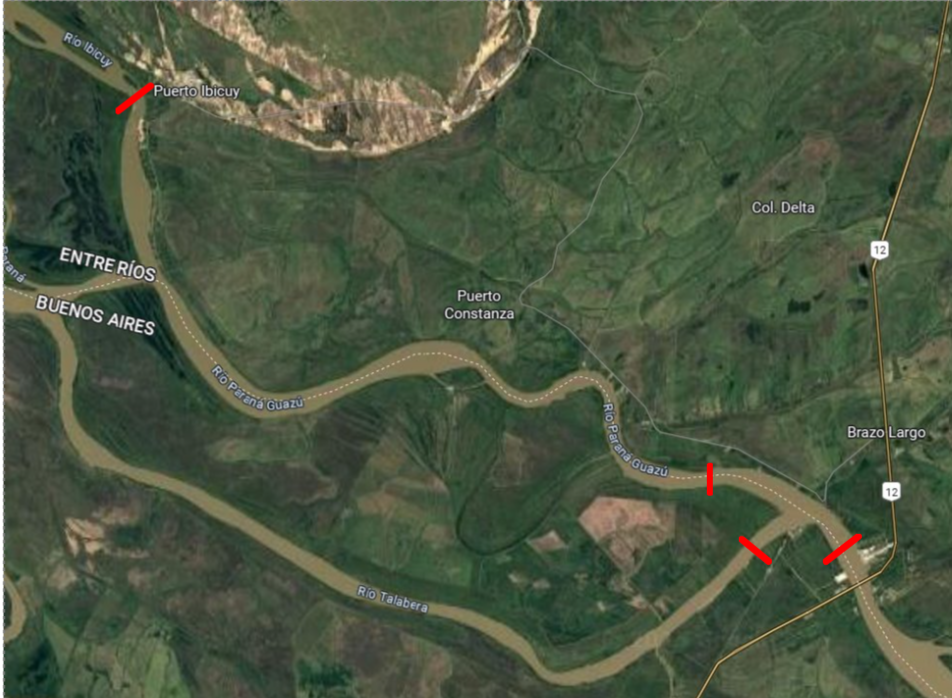
\includegraphics[width=0.5\linewidth]{figures/ch4/Critical measurement points.png}
%     \caption{Critical Cross Section Measurements}
%     \label{fig:fieldwork cross sections}
% \end{figure}

% The program of the boat days consisted of going over the indicated critical cross sections (in red on Figure 4.2) a total of 4 times, using the equipment of INA to save the necessary information of the river. 

The first measured type of data is the flow velocity profile of the river. This was recorded by a SonTek RiverSurveyor M9 Acoustic Doppler Current Profiler (ADCP). This device consists of two components both placed on a floating board held next to the boat while advancing. The components are a vertical acoustic echo sounder beam placed on the back end of the floating board, and a rectangle shape box containing a microprocessor that computes the data on the front end of the board, as seen in Figure \ref{fig:SonTekmeasurement}.

\begin{figure}[H]
    \centering
    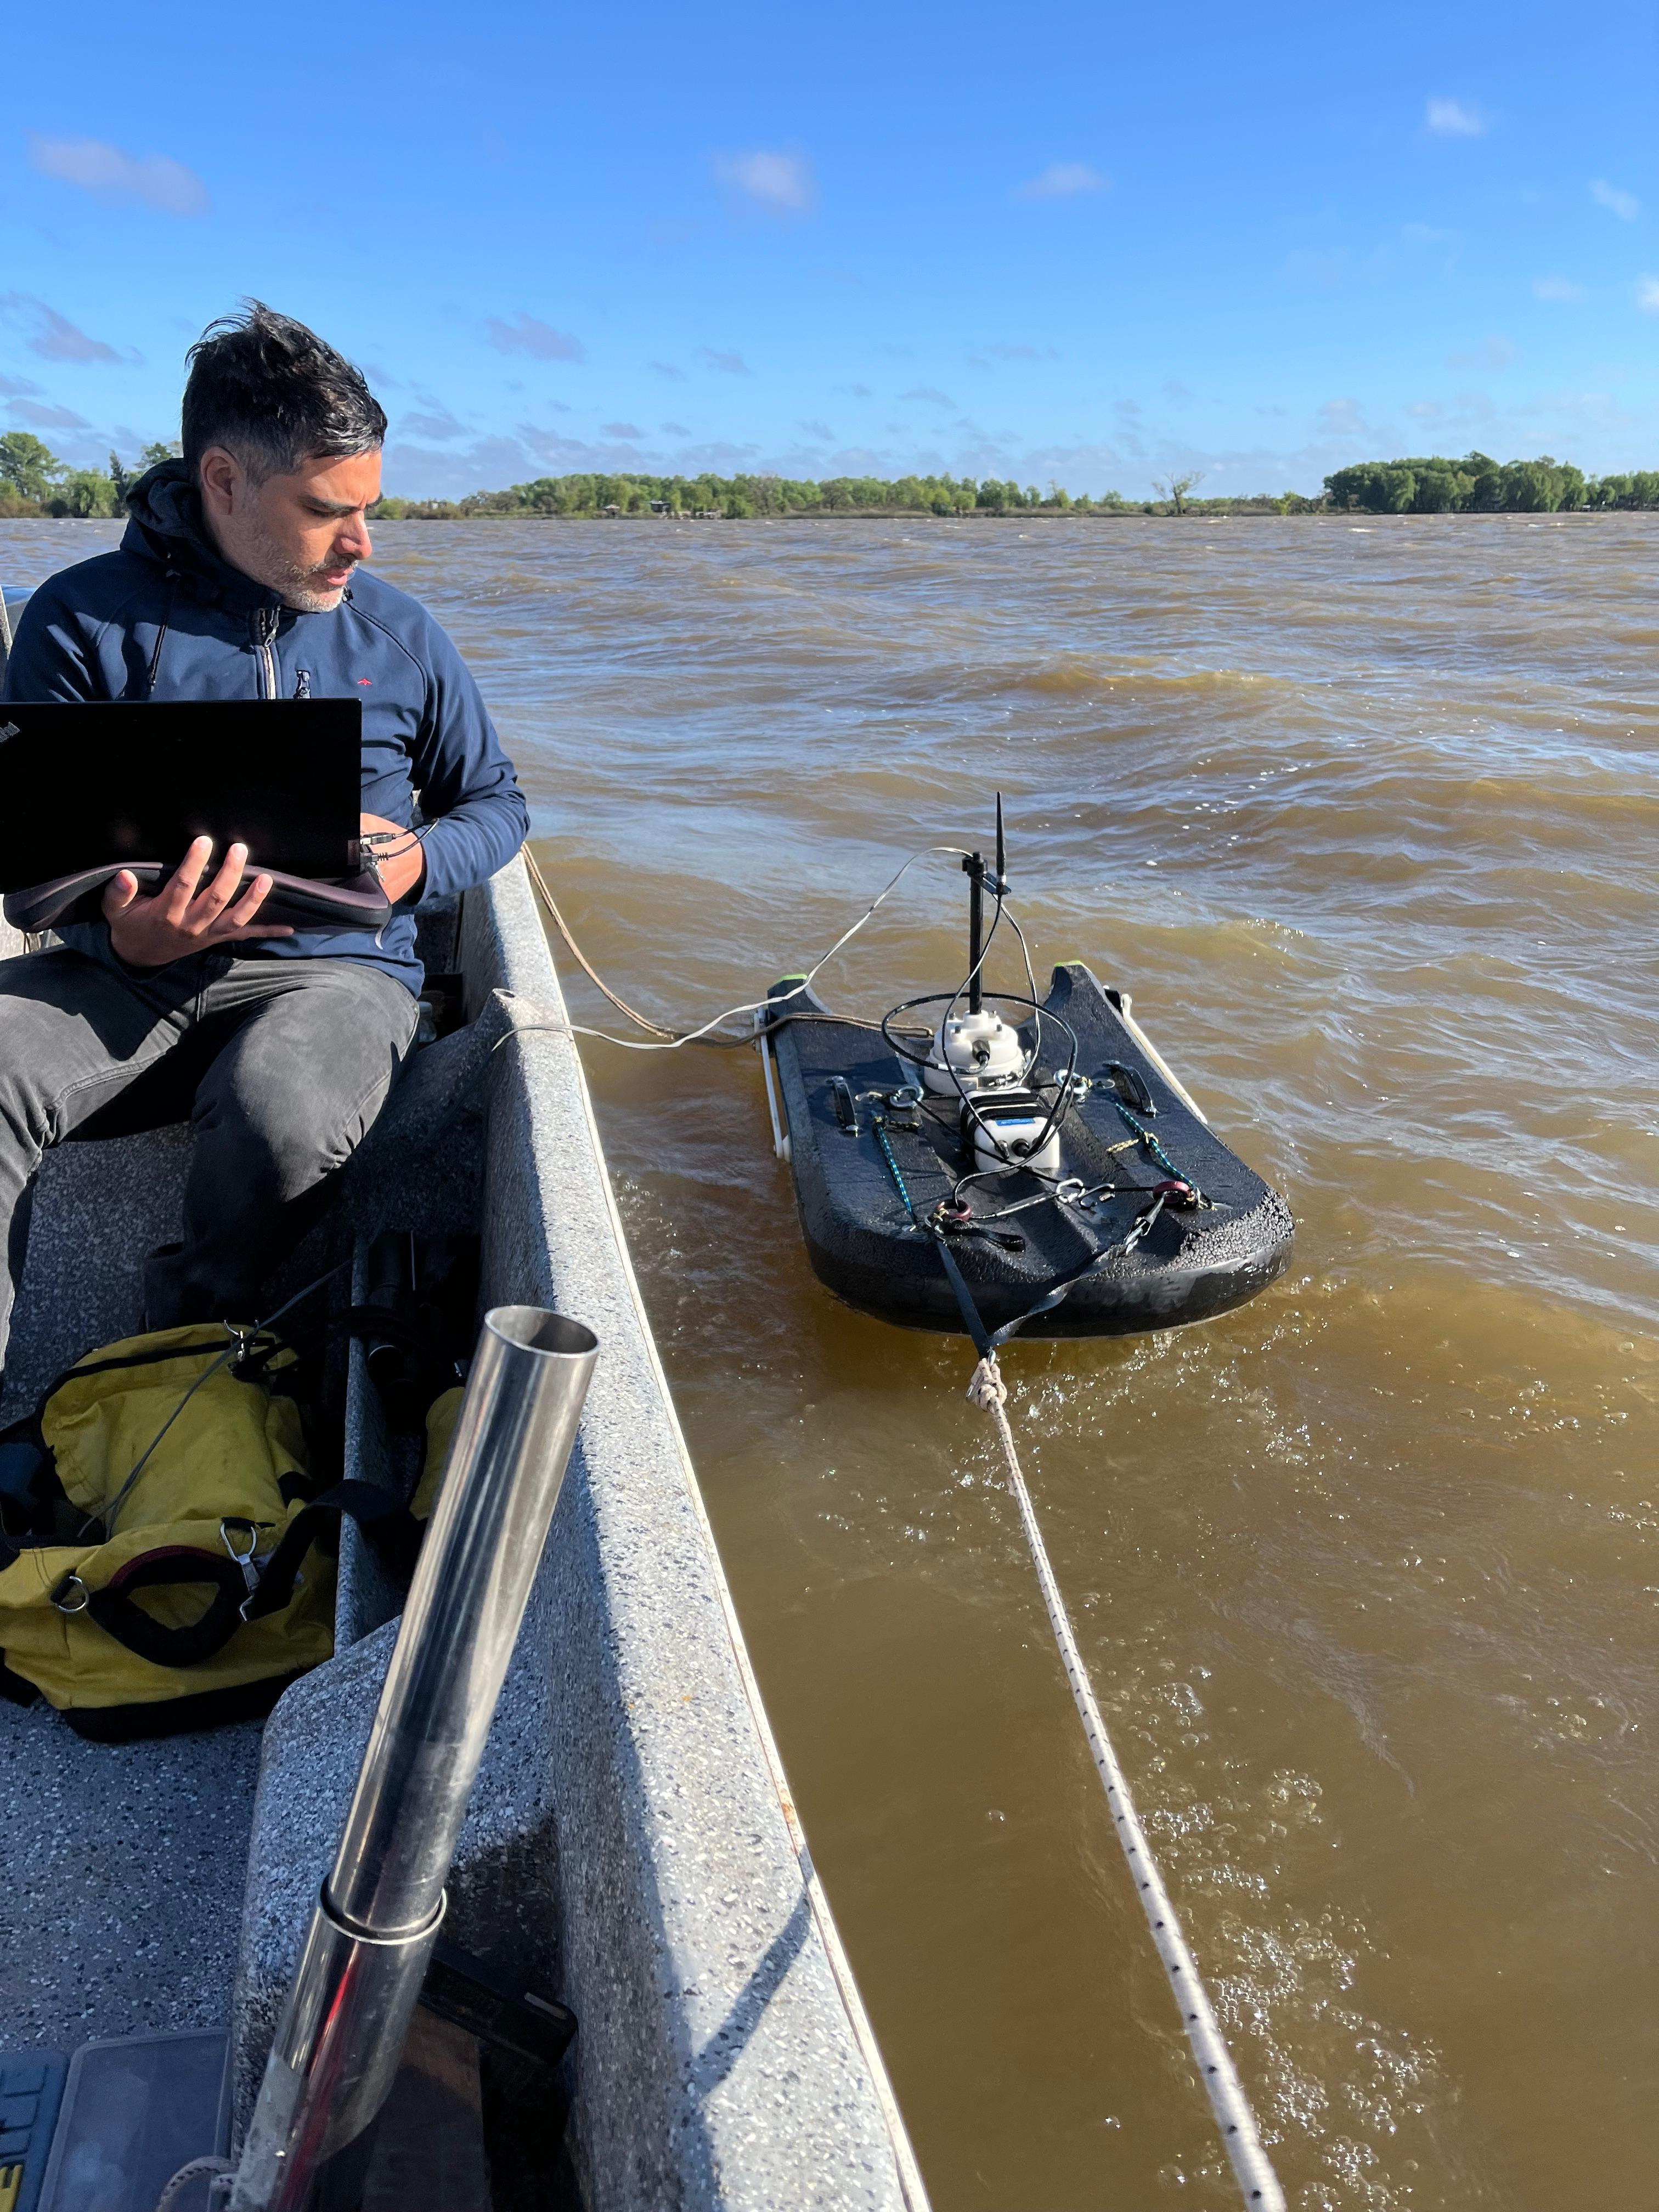
\includegraphics[width=0.5\linewidth]{figures/ch4/sonteknico.jpg}
    \caption{SonTek M9 installed in the field}
    \label{fig:SonTekmeasurement}
\end{figure}

The speciality of the SonTek M9 is that it uses multiple acoustic frequencies to find a high resolution range of depths and flow velocities, while still tracking the geo-referenced position of the vessel using GNSS \autocite{xylemSonTekM9}. The flow velocity is expressed in the form of a vector and the significance of this data lies in the fact that flow velocity is needed to compute the discharge. 

Secondly, the bathymetry, the depth of a channel at the position of the boat on a given timestep, was recorded by using two different methods: the ADCP and the Garmin echosounder. Moving over the whole width of the channel yielded a longitudinal profile, indicating what depth lies at what coordinate.
The echosounder was attached to a pole on the side of the boat, and dipped into the water while the boat was moving. This pole was connected to the Garmin screen showing depth and bathymetry of the channel, as can be seen in Figure \ref{fig:Garmin}. In addition, this screen allowed for monitoring of possible disruption of the river bed. The profile was taken on the whole trajectory between Puerto Guazú to Ibicuy in both upstream and downstream directions. The profile is shown in Figure \ref{fig:measurements day2}.

\begin{figure}[H]
    \centering
    \begin{subfigure}[b]{0.48\textwidth}
        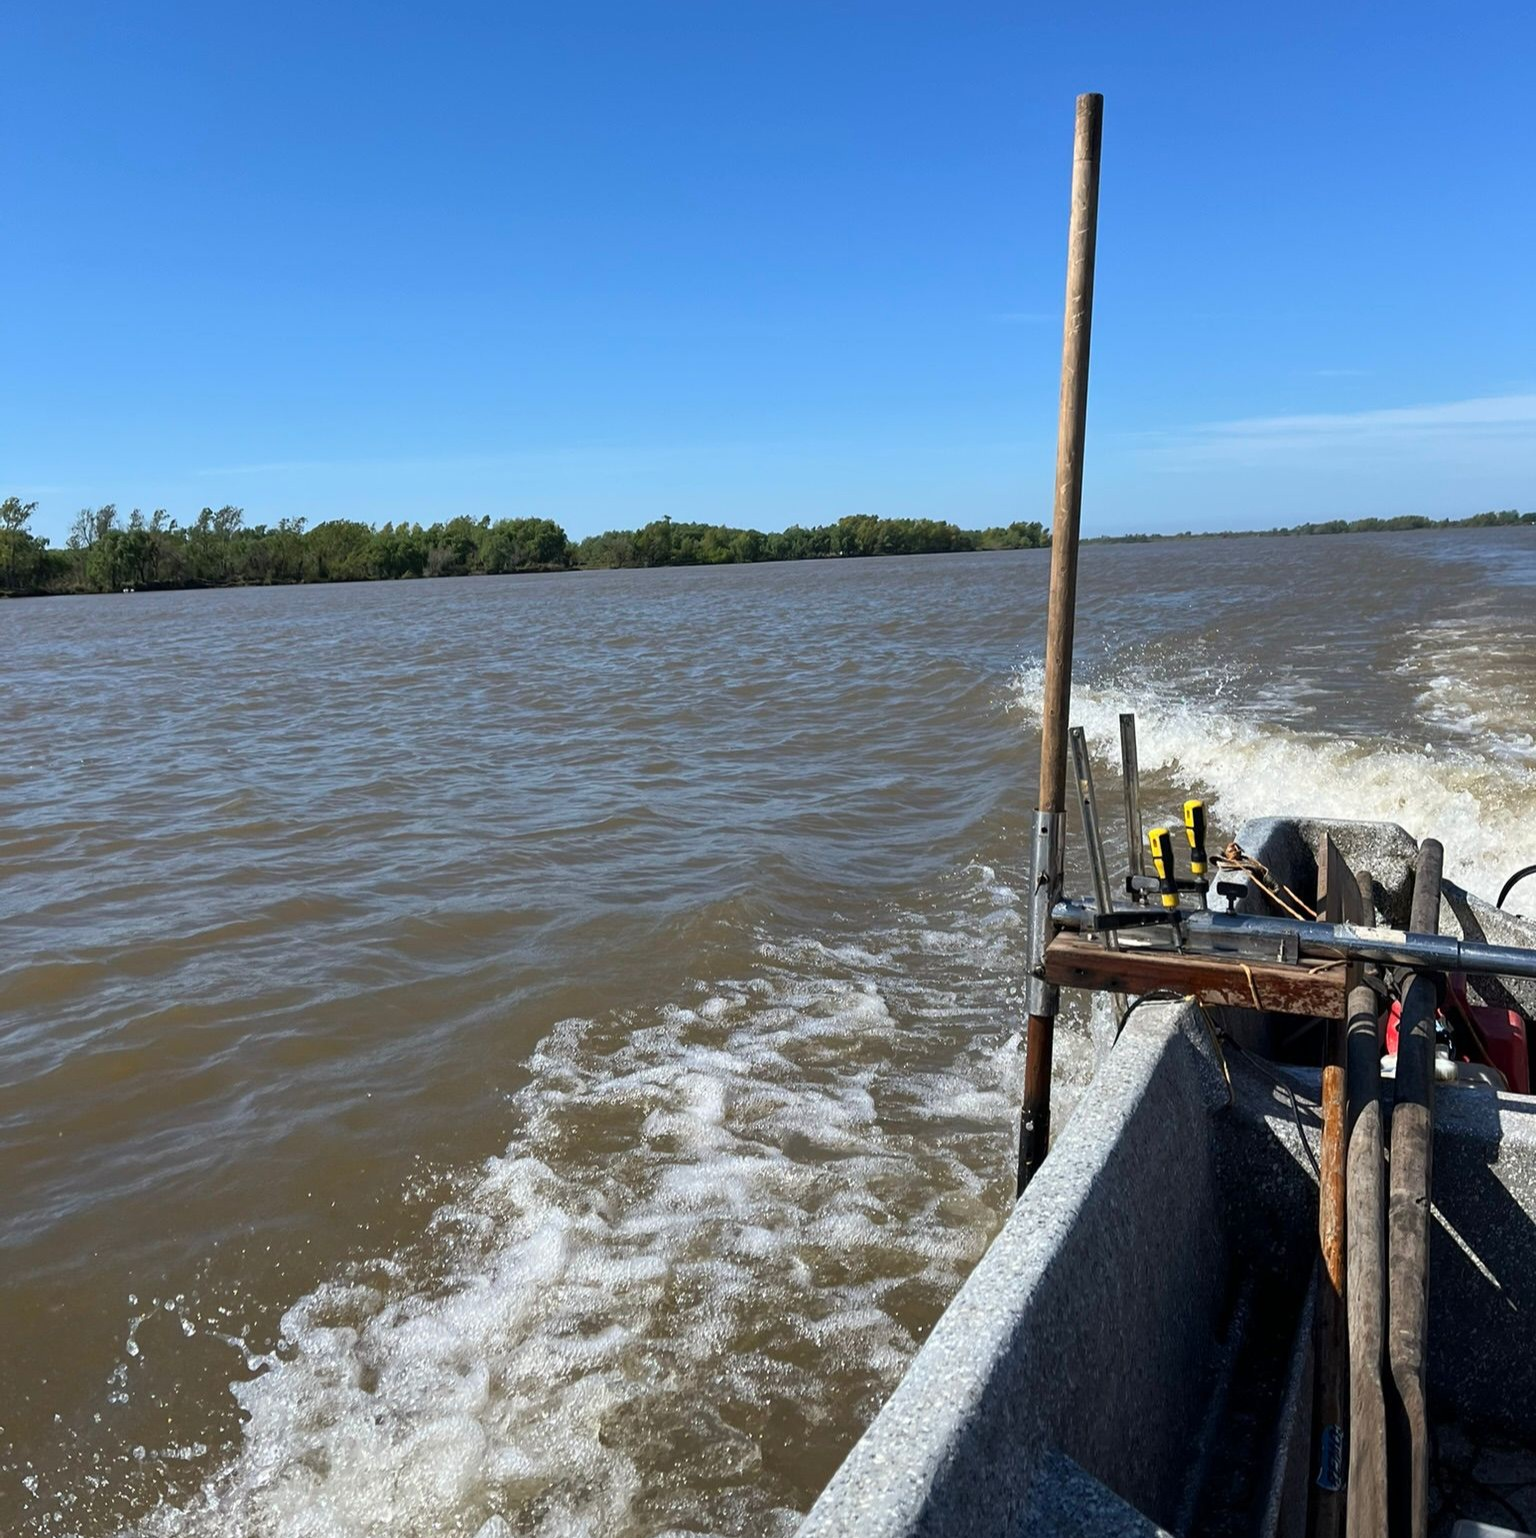
\includegraphics[width=\linewidth]{figures/ch4/Echosounder.jpg}
        \caption{Echosounder attached to boat}
        
    \end{subfigure}
    \hfill
    \begin{subfigure}[b]{0.48\textwidth}
        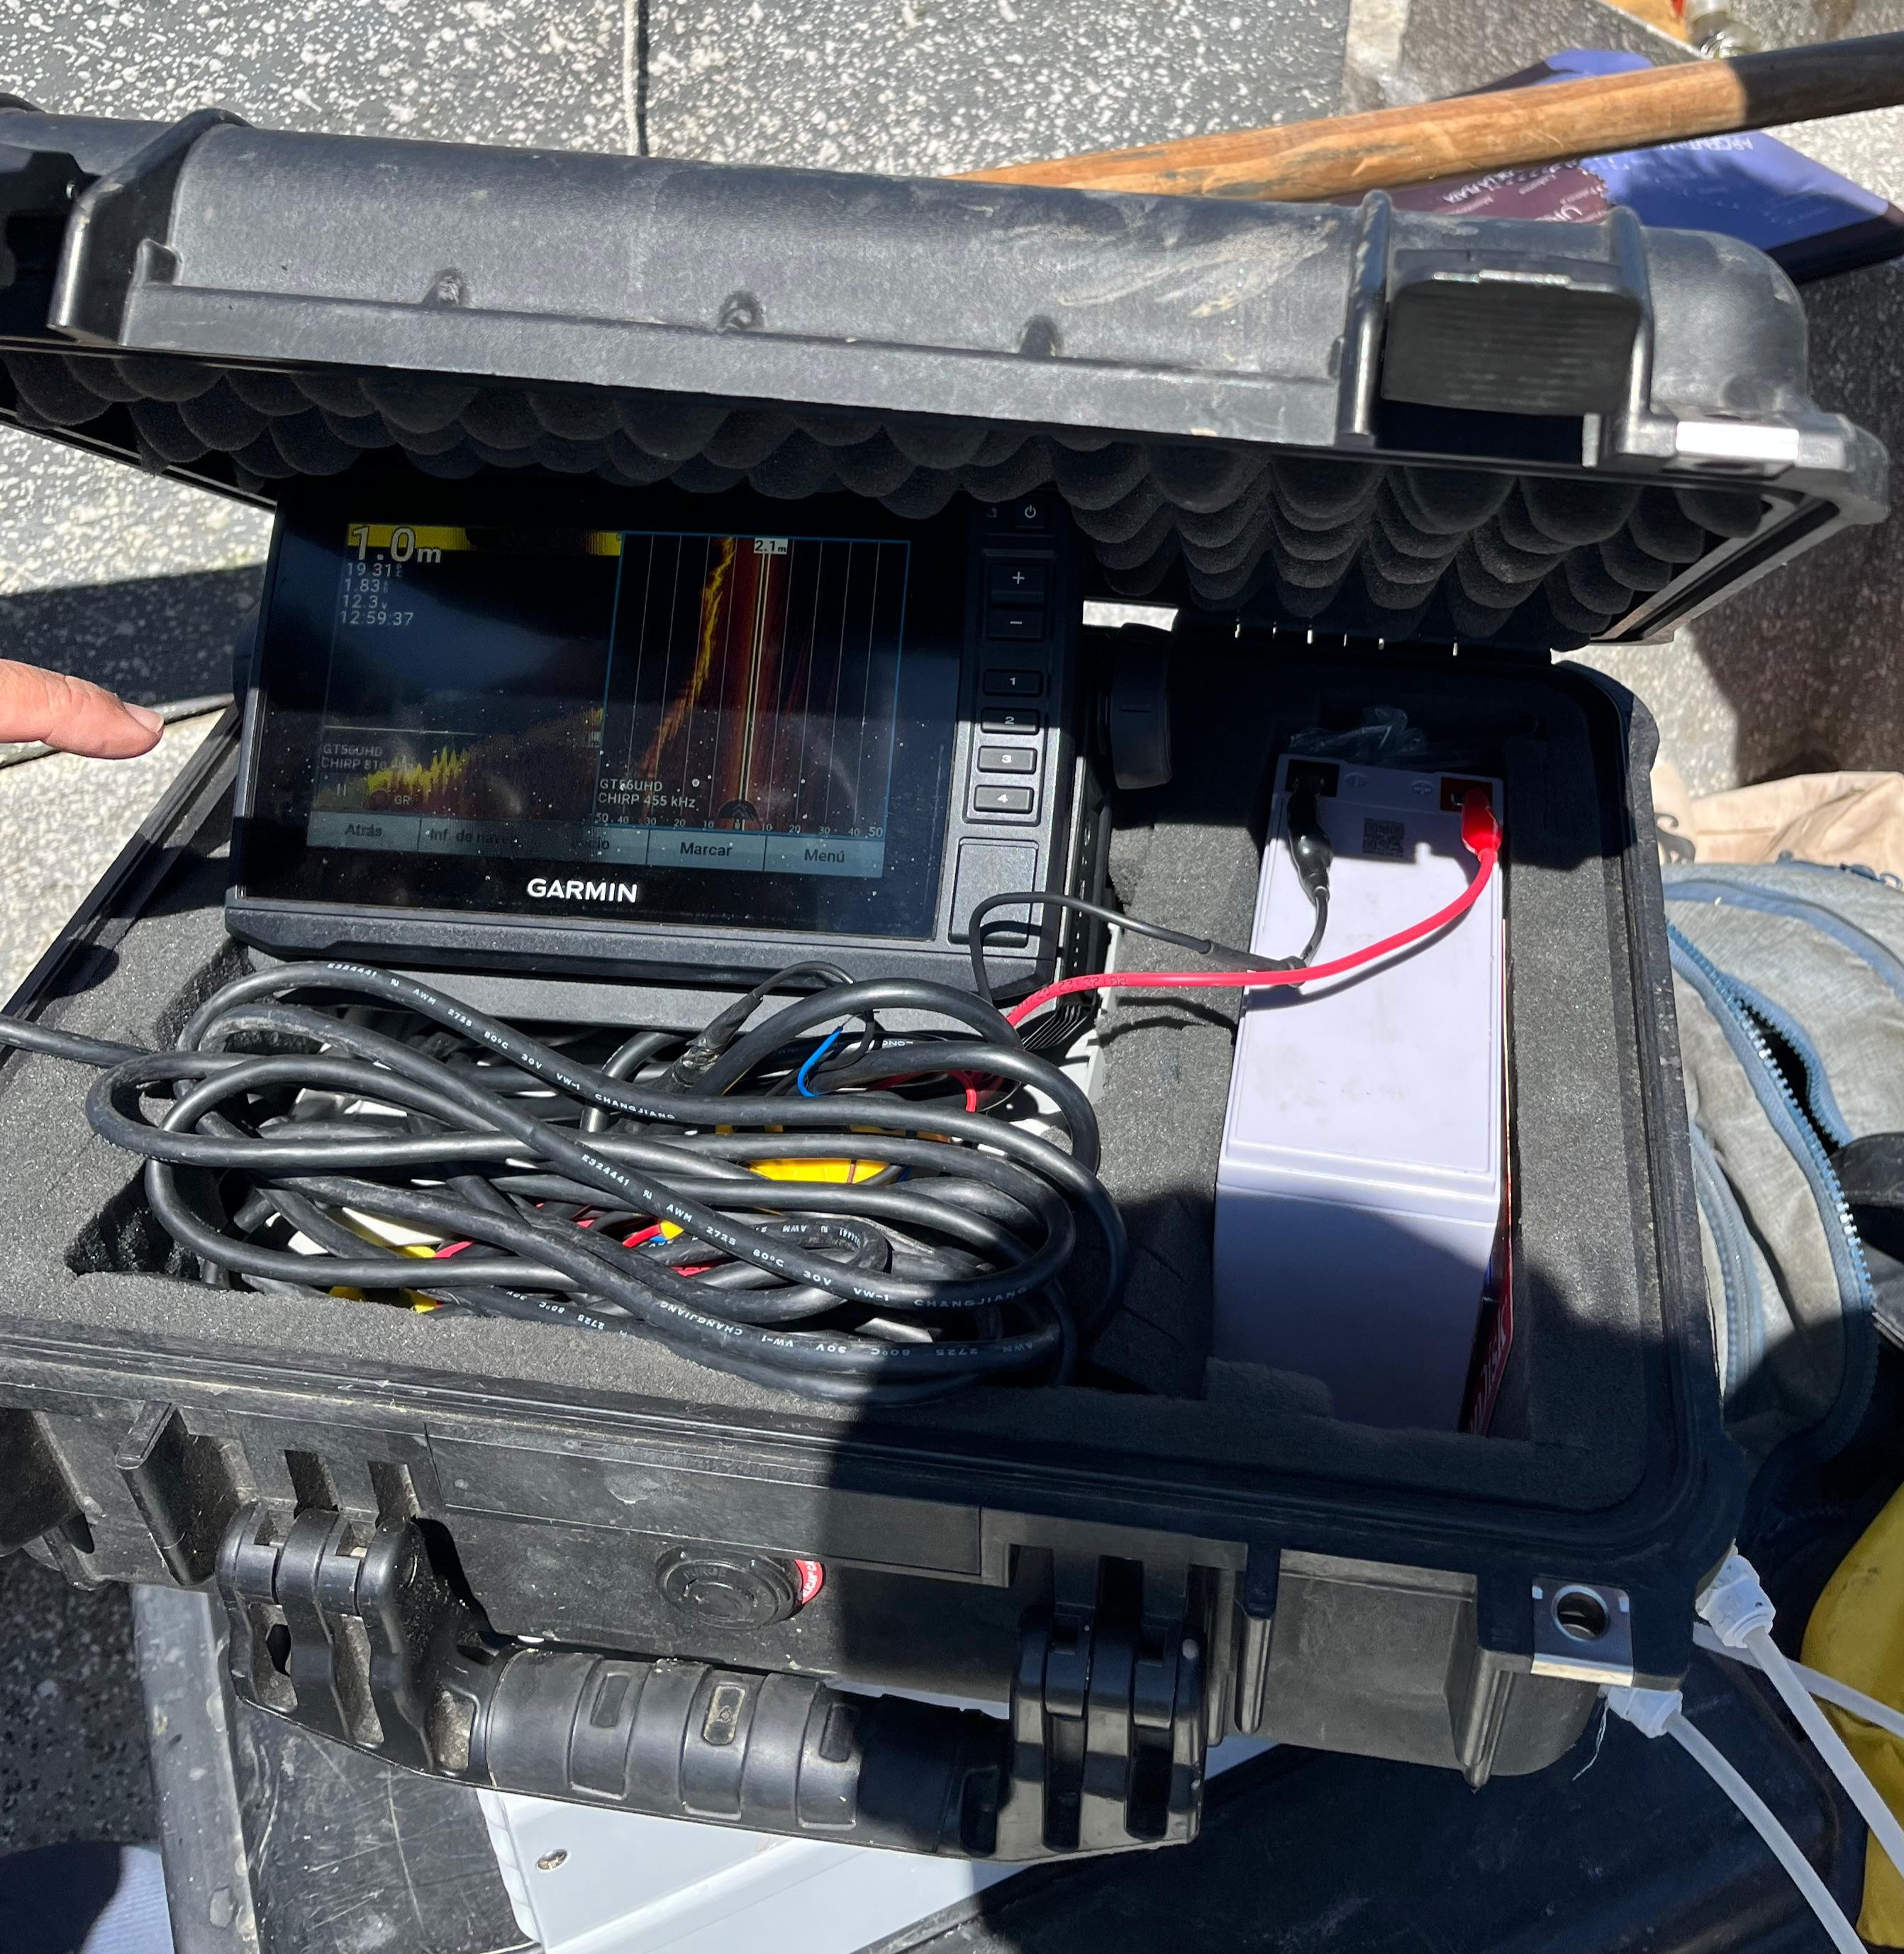
\includegraphics[width=\linewidth]{figures/ch4/garmin.jpg}
        \caption{Garmin material}
        
    \end{subfigure}
    \caption{Echosounder and Garmin measurements}
    \label{fig:Garmin}
\end{figure}

From the bathymetry and flow velocity, the discharge can be determined. The flow velocity \(\mathbf{v}\) was integrated over the depth and width of the channel (through a cross-section) which in the end yielded the discharge. Equation \ref{eq:discharge_integration} summarizes this procedure.

\begin{equation}
    Q = \iint_A \mathbf{v} \cdot d\mathbf{A}
    \label{eq:discharge_integration}
\end{equation}

\noindent Where:
\begin{itemize}
    \item \(Q\) is the discharge, cubic meters per second [m\textsuperscript{3}/s];
    \item \(\mathbf{v}\) is the flow velocity vector, meters per second [m/s];
    \item \(A\) is the cross-sectional area perpendicular to the flow, square meters [m\textsuperscript{2}];
    \item \(d\mathbf{A}\) is an infinitesimal area element.
\end{itemize}

The number of measurements required for a single cross section was defined by the variability of the measurements. That is, a minimum of two measurements was carried out, which was deemed to suffice when the second discharge measurement fell within 10\% of the first one. In addition, correct operation of the vessel's velocity was essential for reliable discharge results: it was made sure that the boat speed never exceeded the flow velocity perpendicular to the cross section under consideration. 

% The aim of the fieldwork was to obtain the data of flow velocity and discharge at the three critical points around the bifurcation of interest during different times, one in the morning and in the afternoon. Consequently this would indicate some changes in discharge for different times, flows, circumstances hence solidifying our data base of examples. 

Further, data was gathered on the suspended sediment concentration of the river. This was done by collecting water with the help of an APEMA BS6A peristaltic pump connected to two plastic tubes. The first tube was short and was used to insert water into the plastic bottles on the boat. The second, long, tube was connected to a weight, which could be lowered into the river until a certain depth. At the desired depth, the fluid was pumped to the surface and collected in the plastic bottles. Then, samples were sealed in order to be sent to the water quality lab in the hydraulic section on the INA site, as seen in Figure \ref{fig:suspended-sediment}. Here, concentrations of fine sediments were determined for all samples. The evolution of the concentrations along the study area is studied in Chapter \ref{chap:hydroanalysis}.

\begin{figure}[H]
    \centering
    % Left image
    \begin{subfigure}[t]{0.48\textwidth}
        \centering
        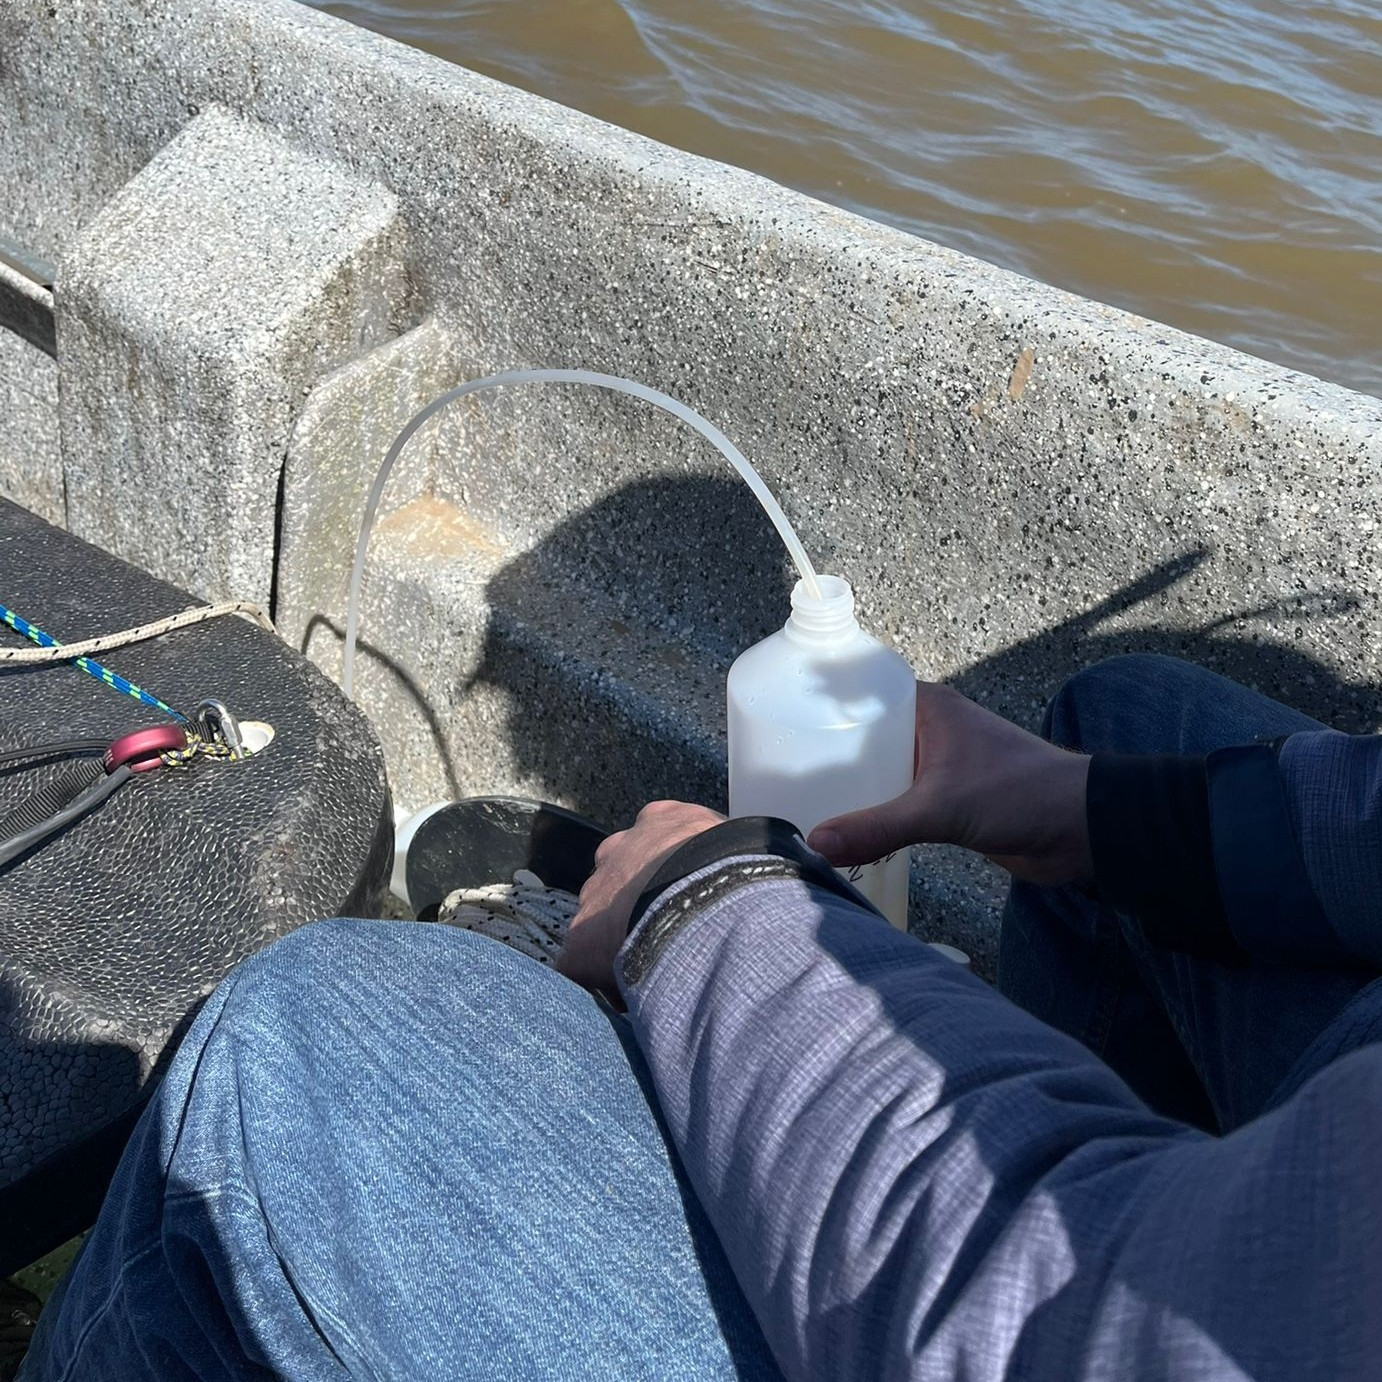
\includegraphics[width=\linewidth]{figures/ch4/fles.jpg}
        \caption{Filling the samples}
    \end{subfigure}
    \hfill
    % Right image
    \begin{subfigure}[t]{0.48\textwidth}
        \centering
        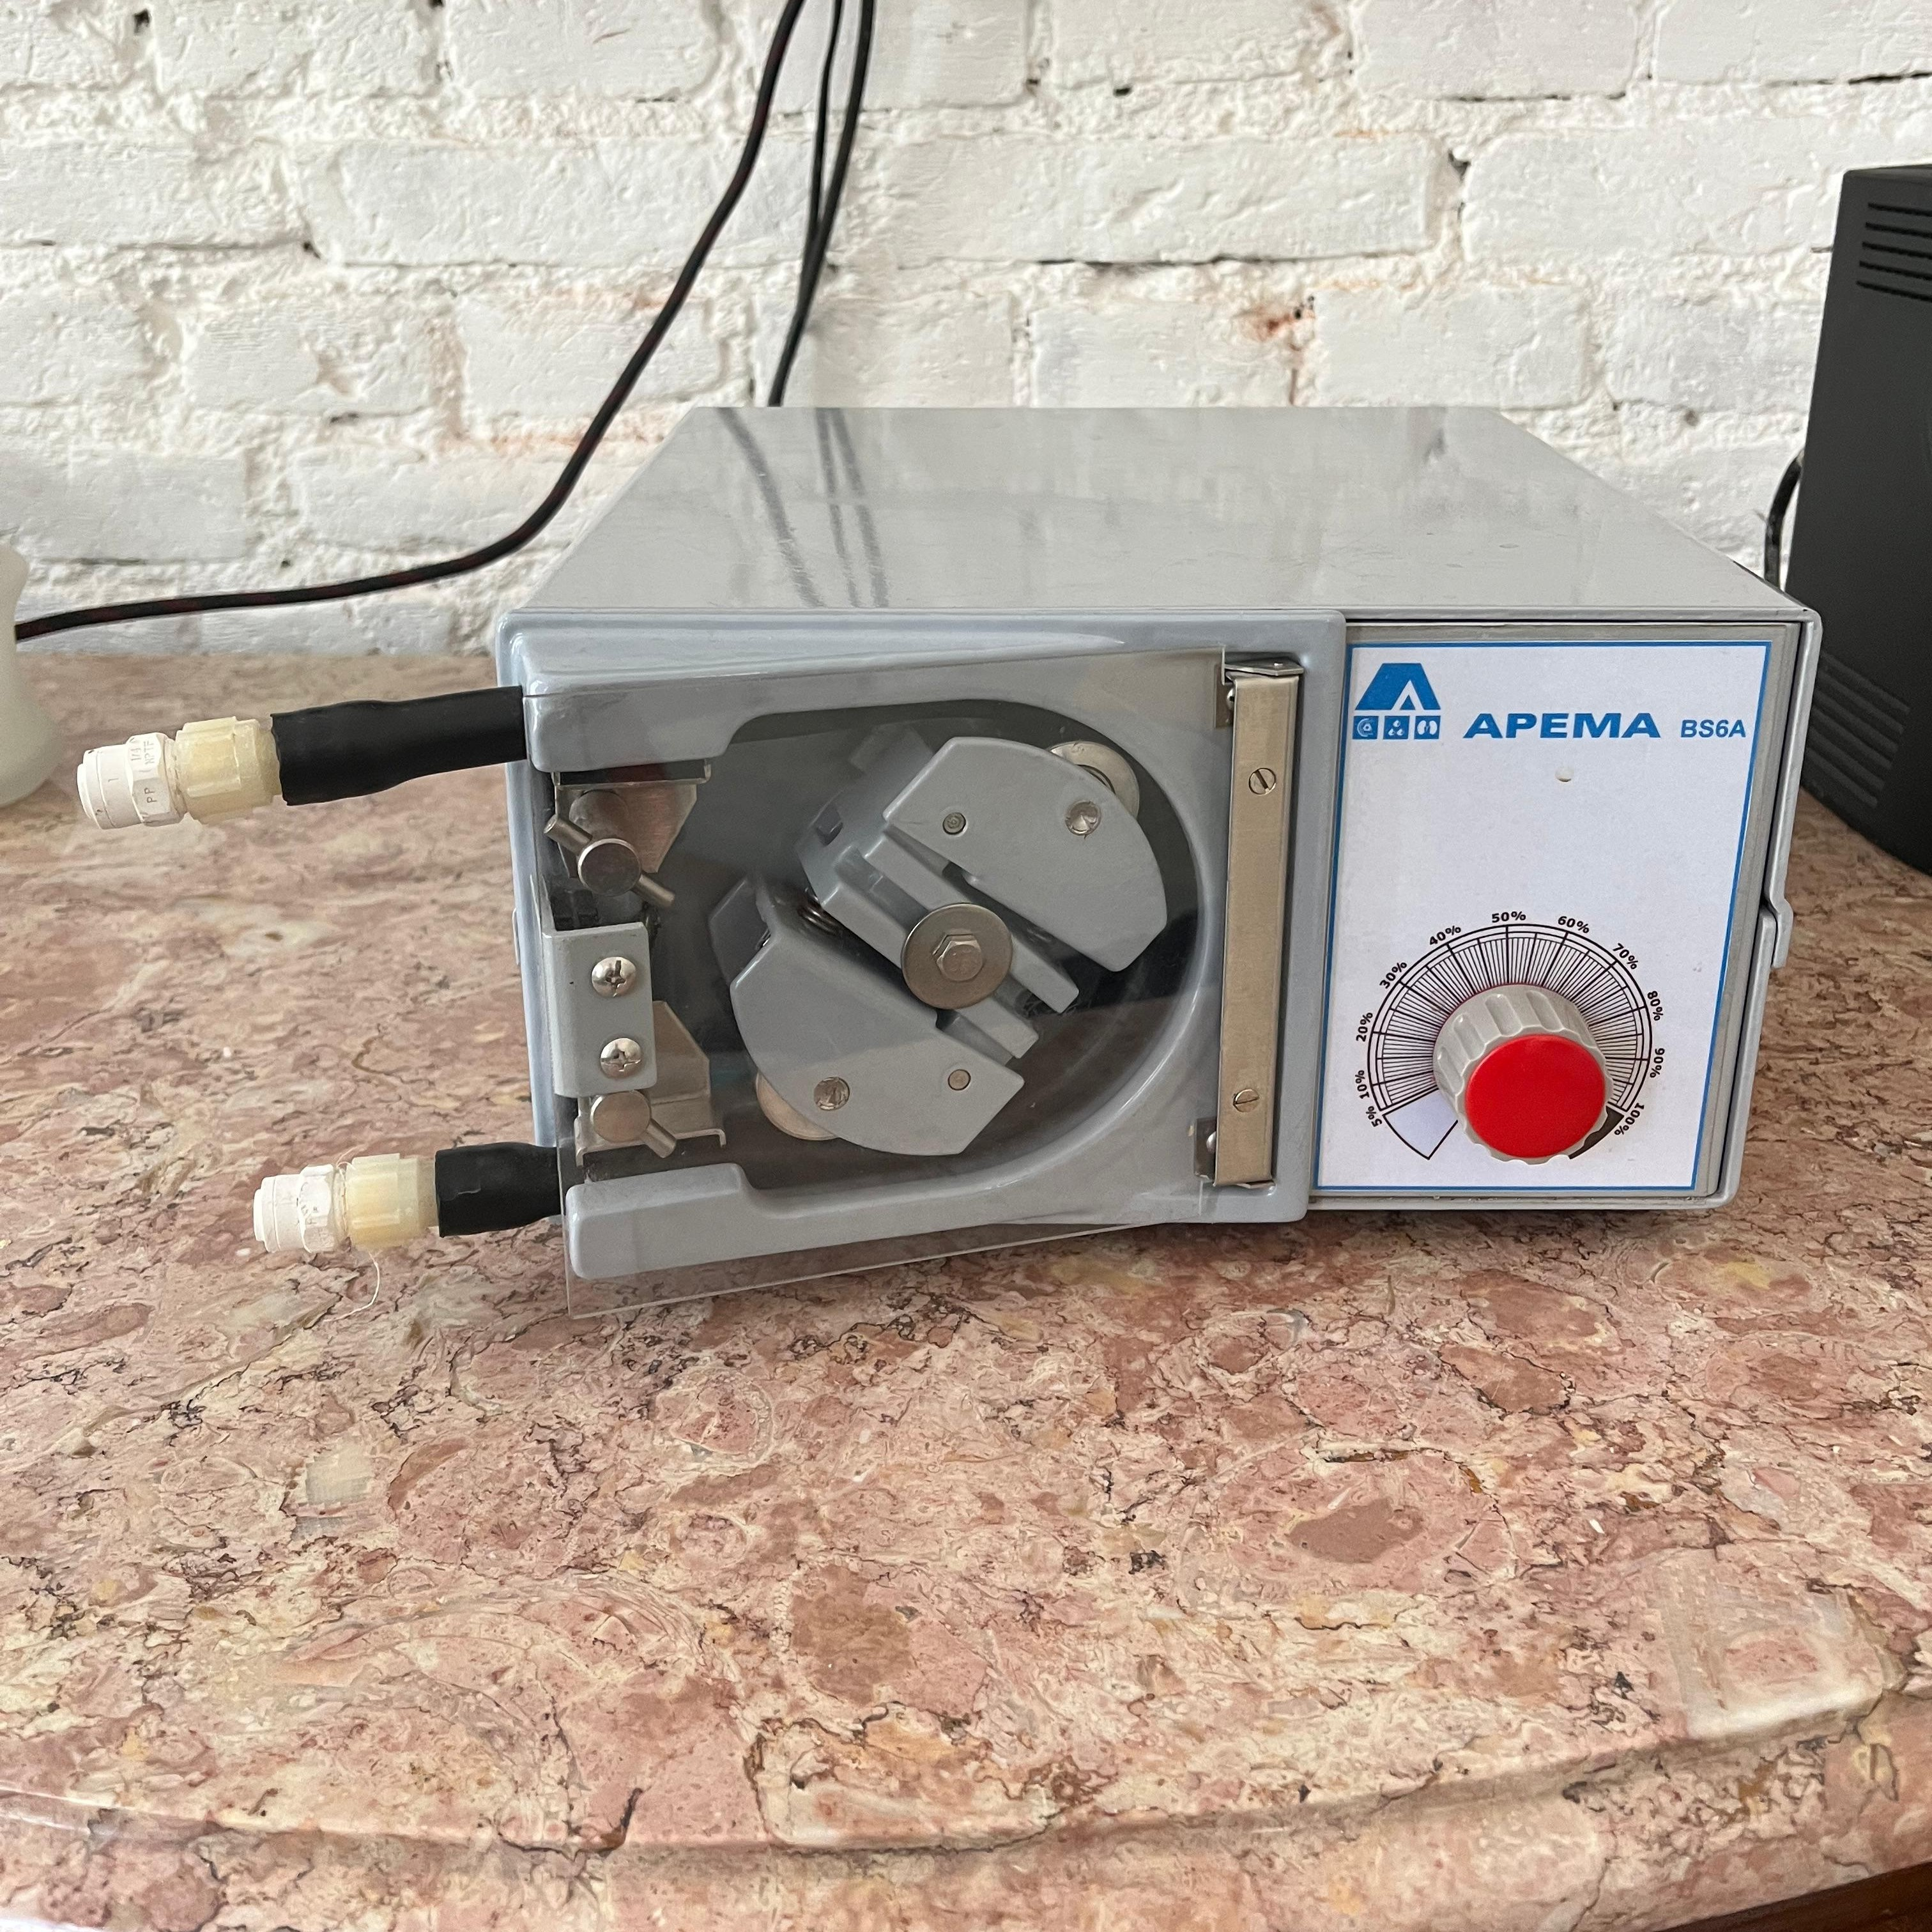
\includegraphics[width=\linewidth]{figures/ch4/APEMA BS6A.jpg}
        \caption{APEMA BS6A device}
    \end{subfigure}
    \caption{Suspended sediment measurements}
    \label{fig:suspended-sediment}
\end{figure}

% In theory, since it was done at different levels of the river, it could potentially indicate a change in concentration from one point upper at Ibicuy to Brazo Largo in the southern, lower part of the study area. From this data, the group could draw even further conclusions.

Finally, the bed load was a necessary measurement for a complete analysis. The method used for this parameter was scraping the bottom layer of the channel with a metal shaped container. The goal was to retrieve samples that represent the granulometry of the bed at different depths. 
During the measurements, a rope was tied to the metal container, which was dropped until it reached the local bed. Then, with help of the current and the movement of the boat, the container was dragged along with the horizontal movement and sediment was gradually collected. Once this was done, the rope and the container were pulled up and restored in the boat. The last step was to collect sediment and put it in a plastic bag. These samples were later analysed in the lab. The metal container as well as the sediment samples are shown in Figure \ref{fig:bed-load}.

\begin{figure}[H]
    \centering

    % First (large) image
    \begin{subfigure}{0.7\textwidth}
        \centering
        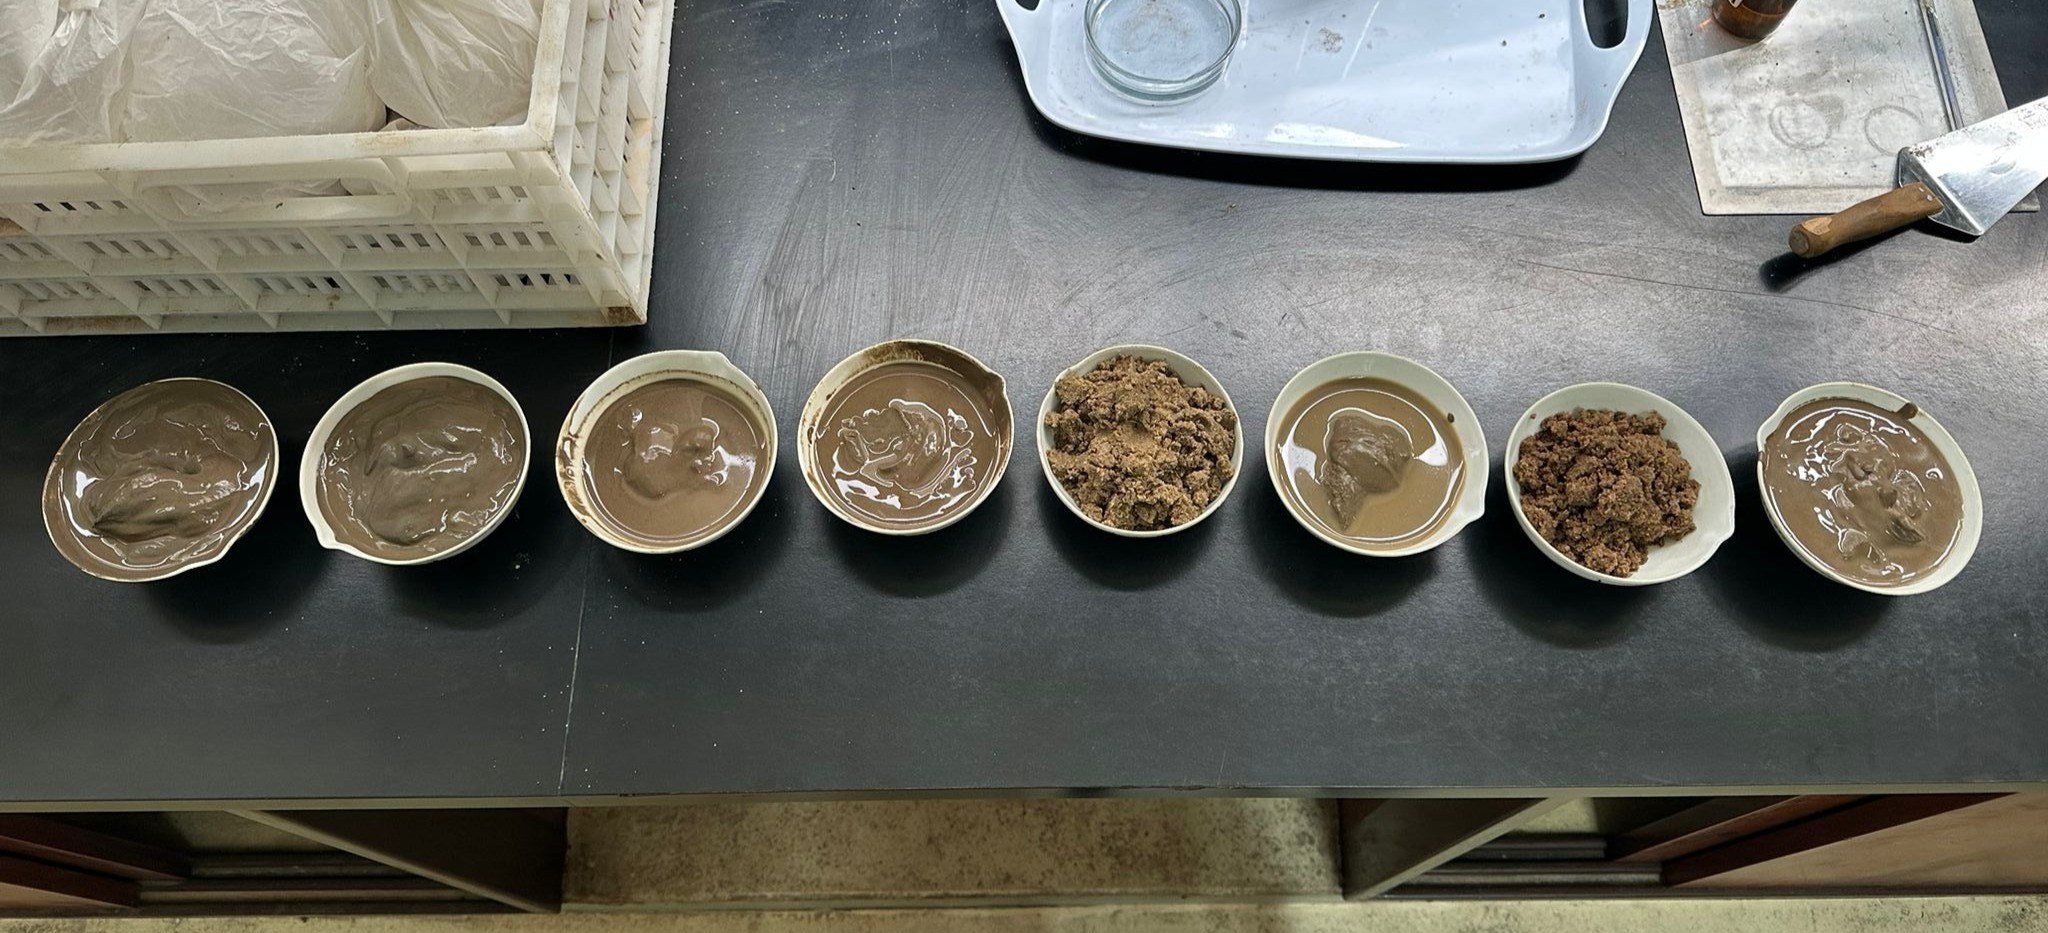
\includegraphics[width=\linewidth]{figures/appendixE/soilsamples.jpg}
        \caption{Bed load samples from the fieldwork}
    \end{subfigure}

    \par\vspace{0.5cm} % use this instead of \vspace alone

    % Two smaller images side by side
    \begin{subfigure}{0.48\textwidth}
        \centering
        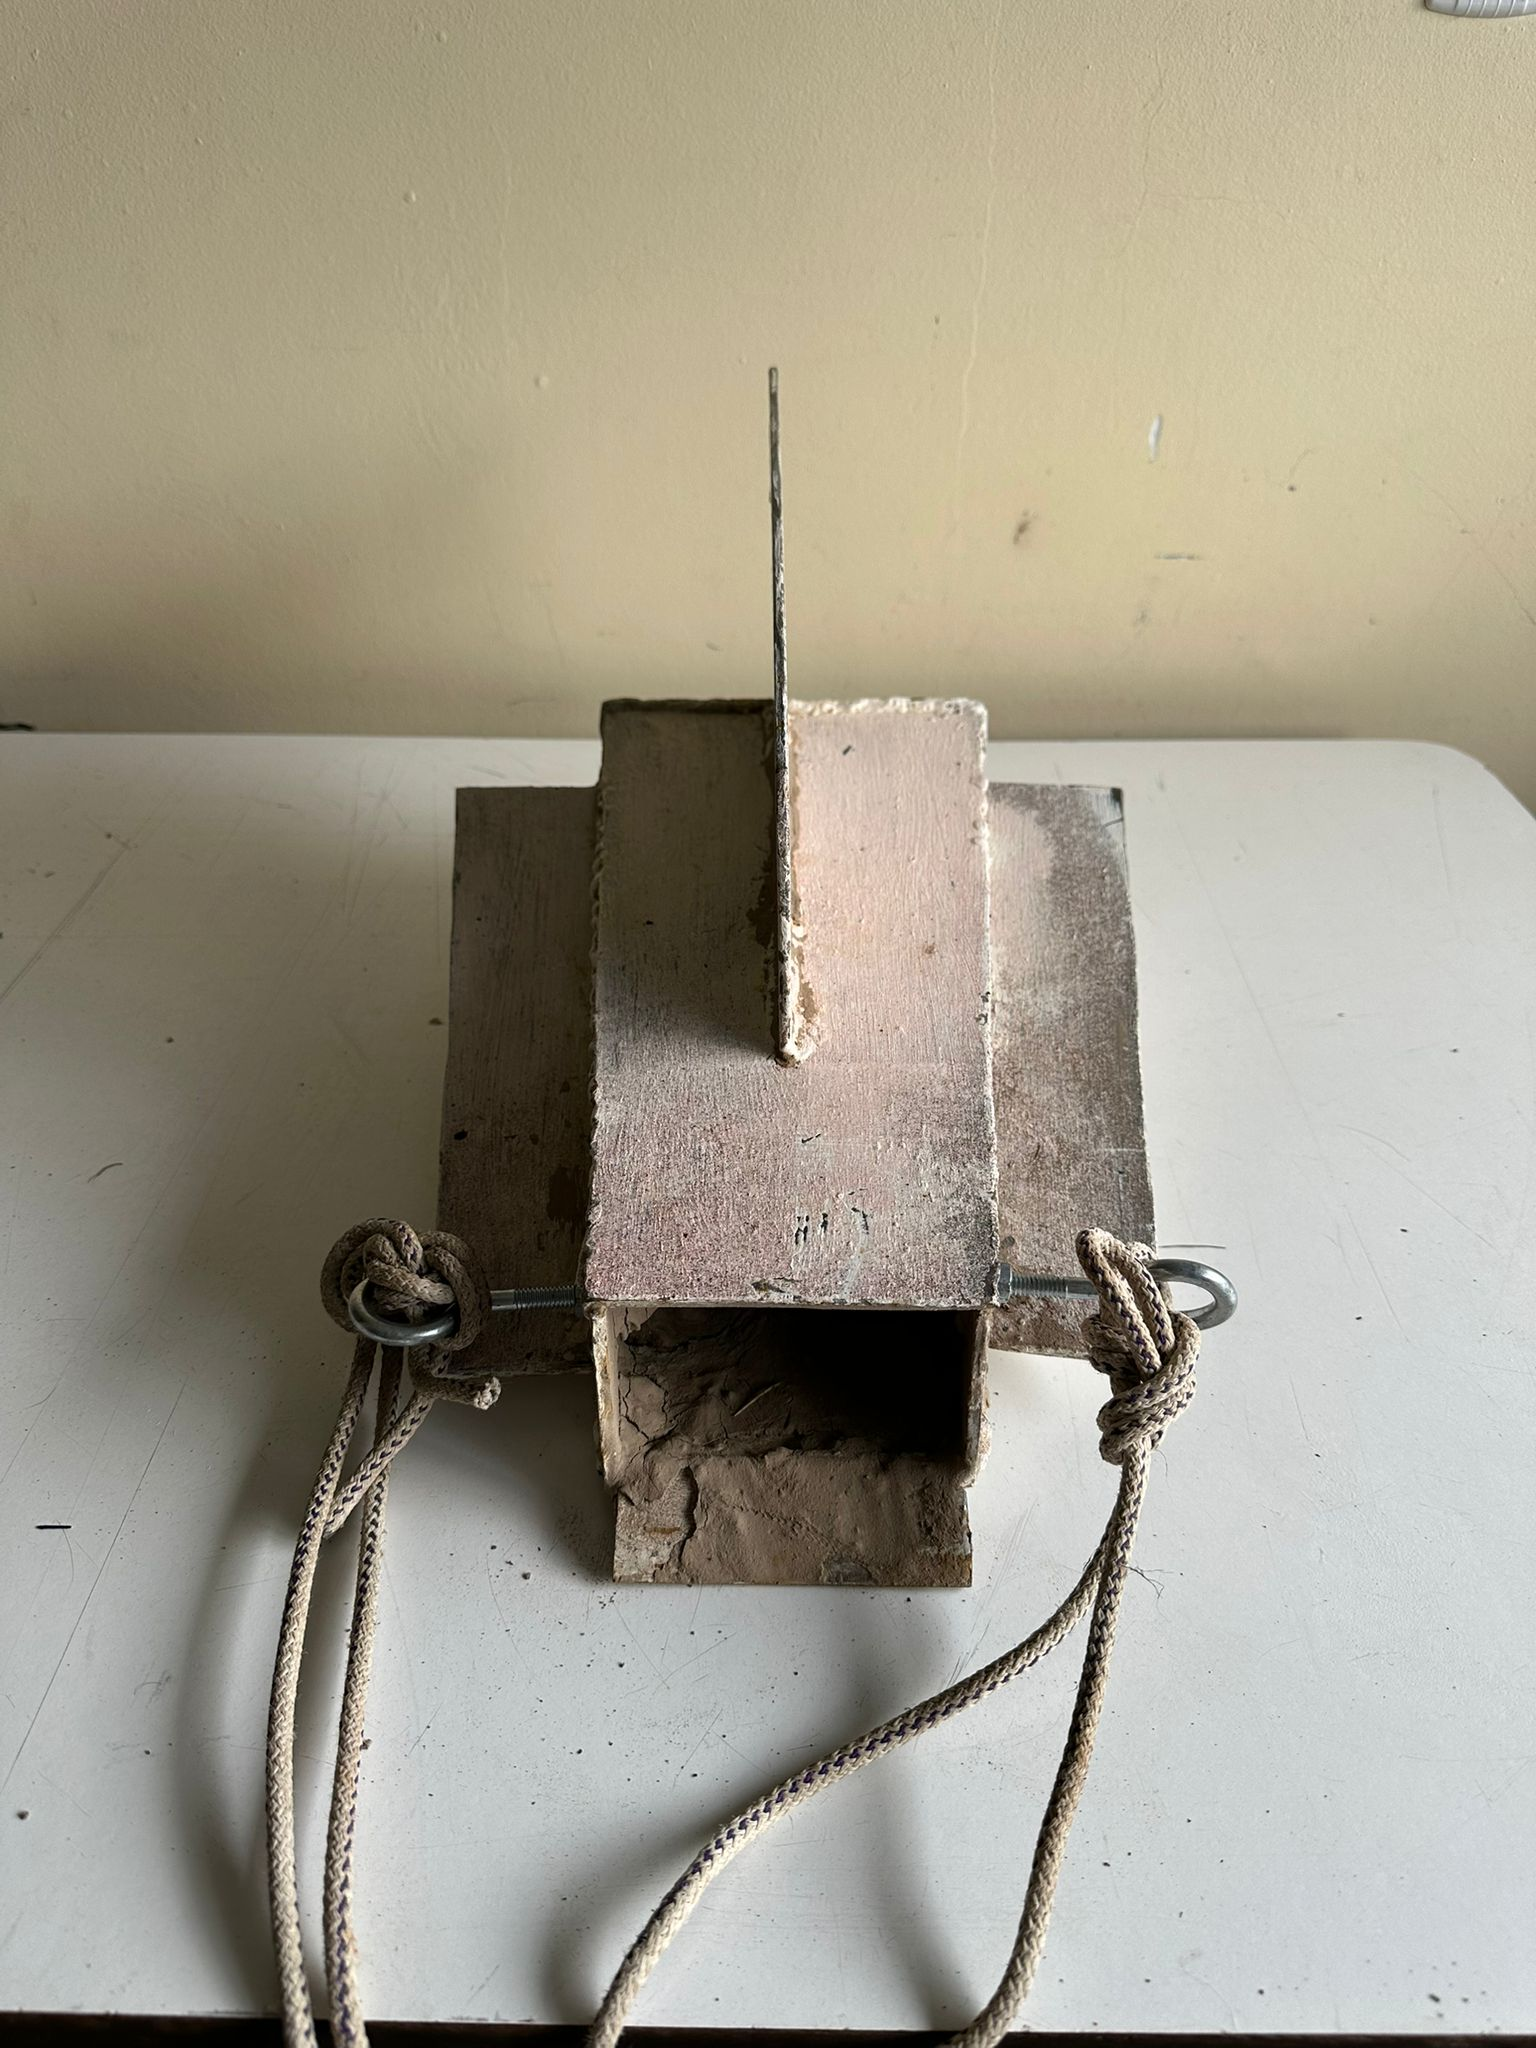
\includegraphics[width=\linewidth]{figures/appendixE/metalcontainer.jpg}
        \caption{Metal container used}
    \end{subfigure}\hfill
    \begin{subfigure}{0.48\textwidth}
        \centering
        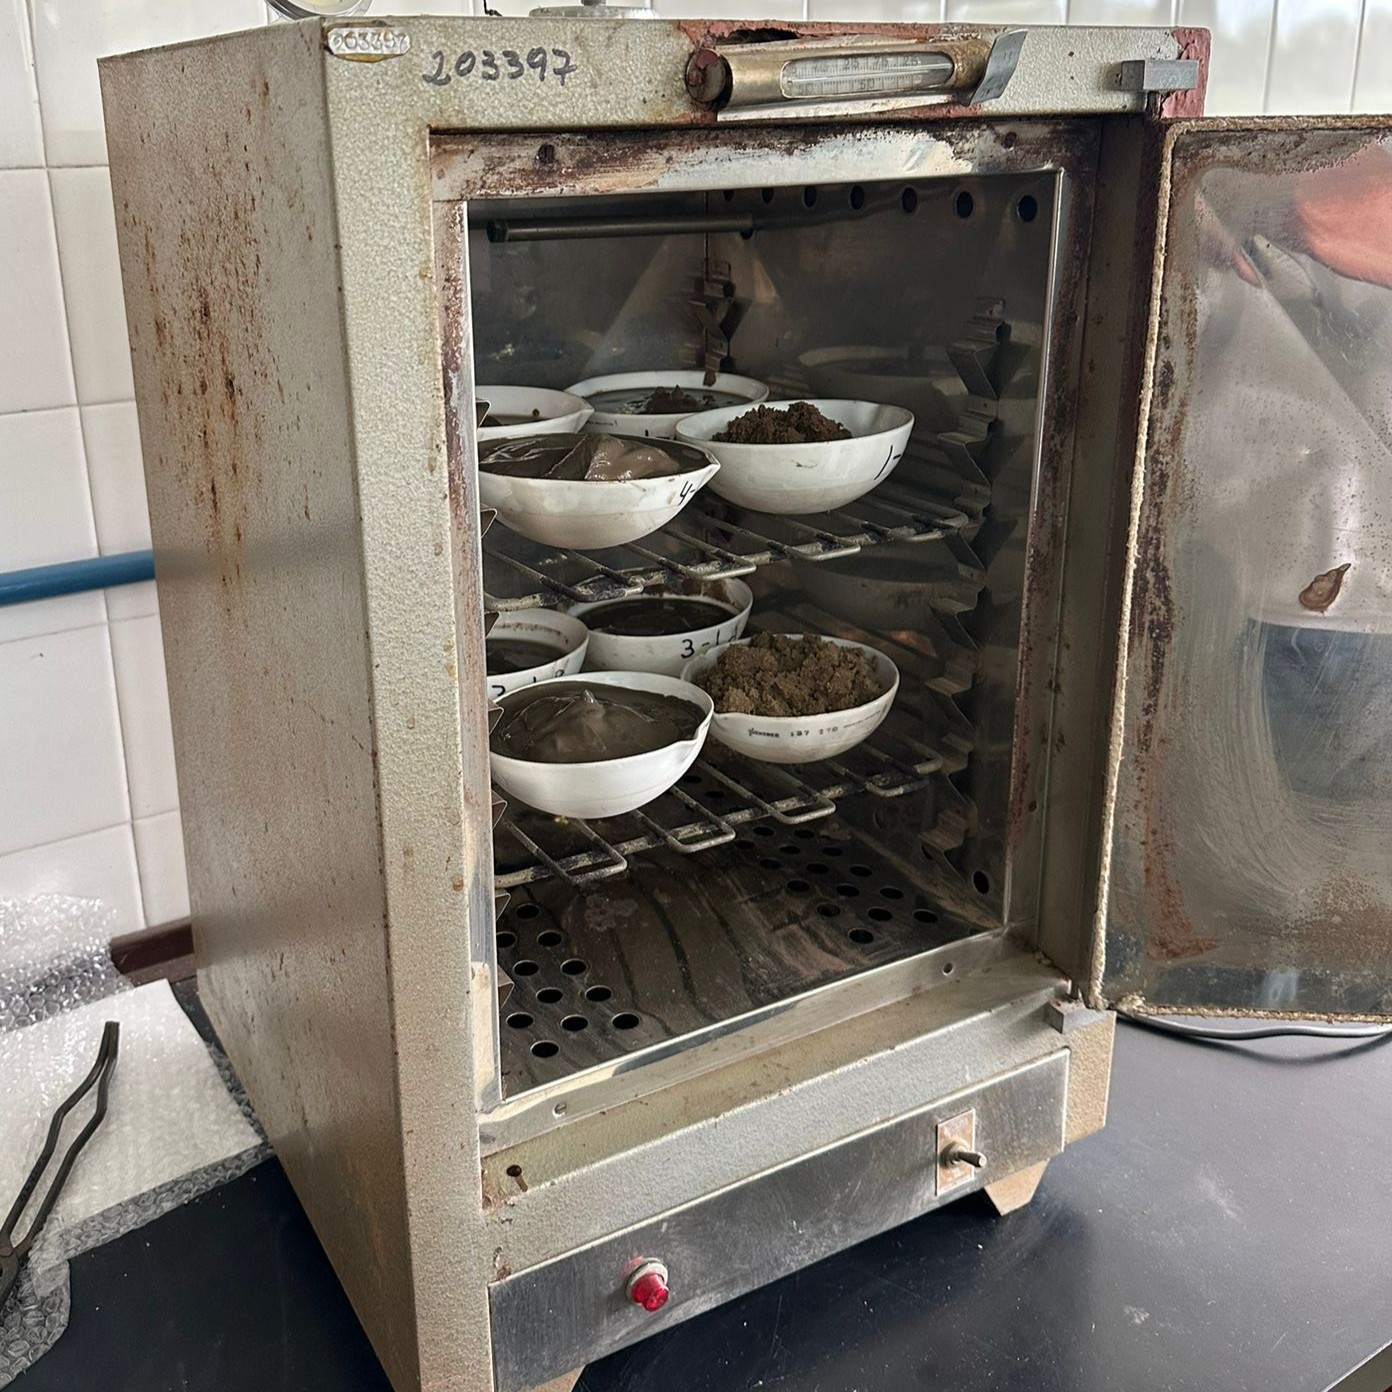
\includegraphics[width=\linewidth]{figures/appendixE/oven.jpg}
        \caption{Oven to dry samples}
    \end{subfigure}

    \caption{Bed load measurements}
    \label{fig:bed-load}
\end{figure}

A total of 7 samples from 4 different locations was collected. The first three locations were the cross sections around the extracting point in the bifurcation of the Paraná Guazú with the Talabera river. For each of these three cross sections, two samples were taken from the soil, one at 10 meters depth and one at 15 meters depth. The final sample was taken at 10 meters depth in the cross section upstream close to Puerto Ibicuy. All samples were sieved with six differently sized sieves, which took 10 minutes per sample. Before sieving, the samples were crushed to prevent particles from clustering. The sieving machine is presented in Figure \ref{fig:siev} and the whole collection of annotated samples can be found in Appendix \ref{appendix:Lab data}.

\begin{figure}[H]
    \centering
    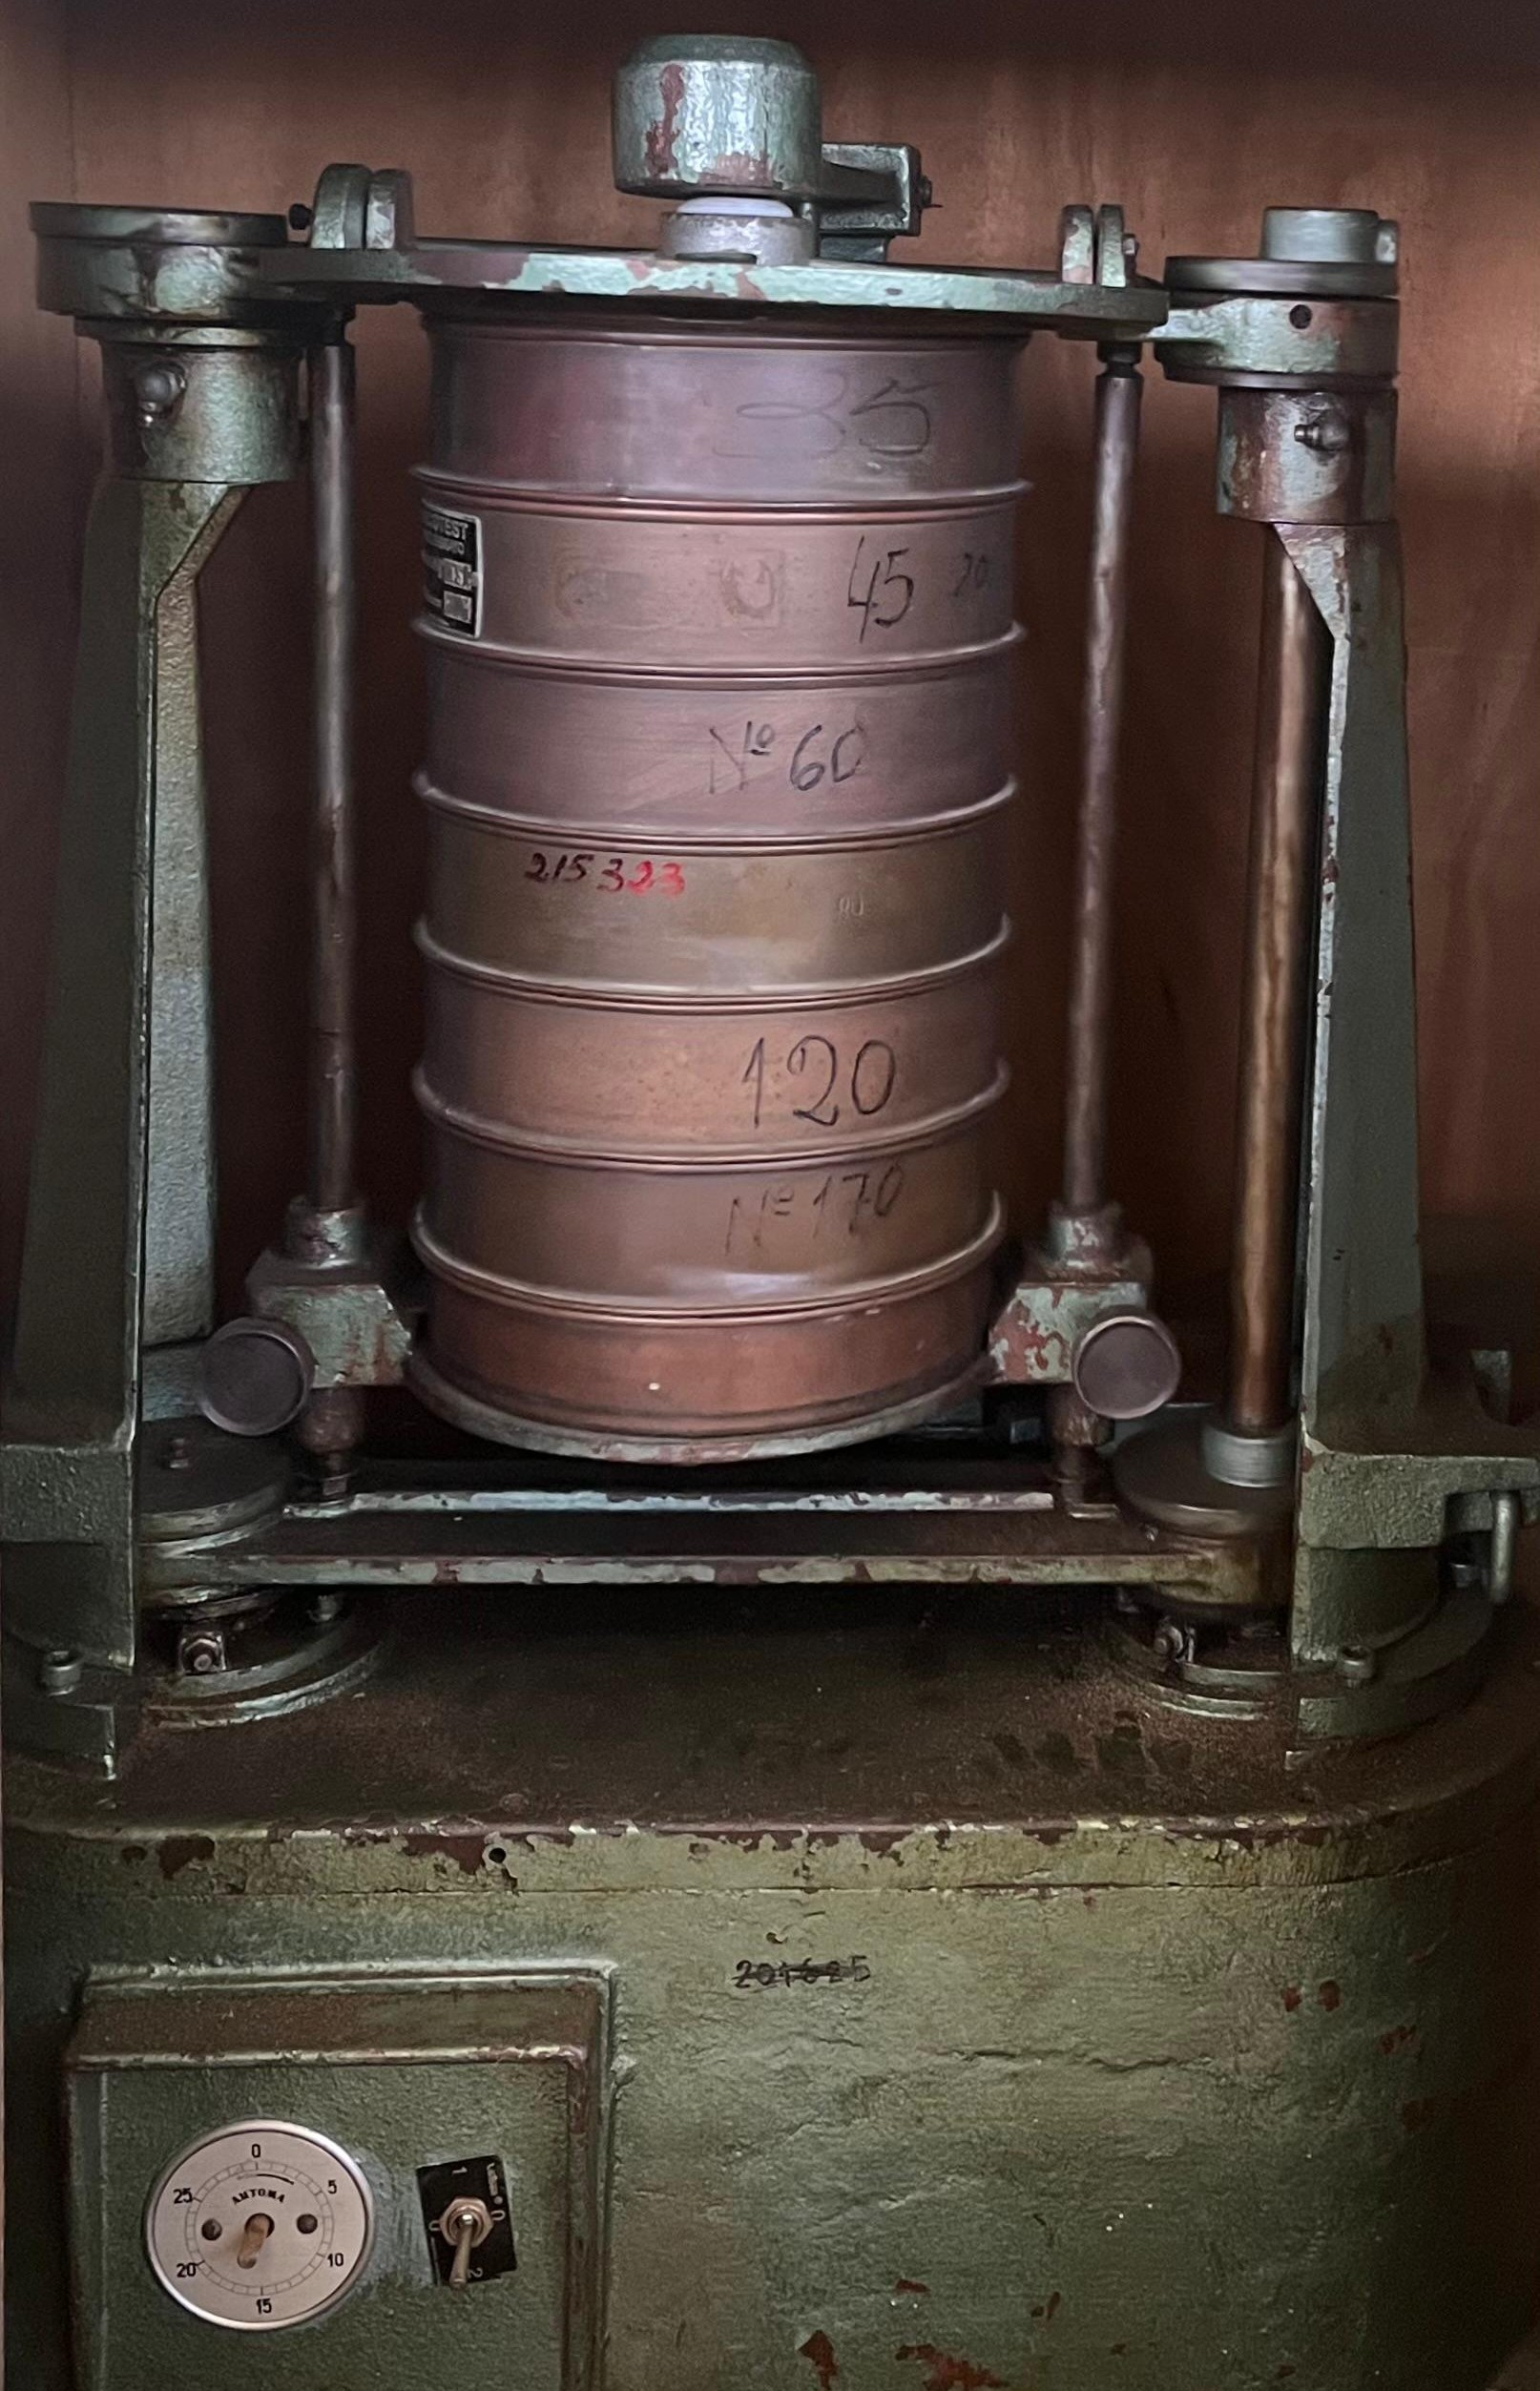
\includegraphics[width=0.35\linewidth]{figures//ch3/siev.jpeg}
    \caption{Sieving machine}
    \label{fig:siev}
\end{figure}

\subsection{Locations of interest}
The measurement campaign was spread out over two main locations. The first location contains a number of cross sections and sediment samples recorded at the confluence of the Talabera and the Paraná Guazú. Figure \ref{fig:measurements day1} shows a summary of the performed measurements. In total, three sections were studied with the following measurements per cross section:
\begin{itemize}
    \item 2 ADCP profiles, yielding bathymetry, discharge and flow velocity;
    \item 2 bed load samples at different locations with different depths;
    \item 5 suspended sediment samples at a single location with varying depths.
\end{itemize}

\begin{figure}[H]
    \centering
    \includegraphics[width=0.70\linewidth]{figures/ch4/day1.png}
    \caption{Measurement location confluence Talabera-Paraná Guazú \autocite{googleGoogleEarth2025}}
    \label{fig:measurements day1}
\end{figure}

\vspace{0.2cm}
The second location contains measurements at Puerto Ibicuy. Here, cross sections were measured in the vicinity of the confluence of the Ibicuy and the Paraná Guazú. In addition, the echo-sounder was active. Its recorded tracks can be found in Figure \ref{fig:measurements day2}. The following results were found for location 2:
\begin{itemize}
    \item 6 ADCP profiles: 2 profiles each for the most upstream and most downstream cross section, respectively. 1 profile for those in between; 
    \item 1 bed load sample near Puerto Ibicuy;
    \item 2 longitudinal profiles along the confluence of Talabera and Paraná Guazú (dredging location), measured upstream and downstream to study dune migration. While navigating, GPS applications were used to make sure the paths were identical (see Figure \ref{fig:longprofiles map}).
\end{itemize}

\begin{figure}[H]
    \centering
    \includegraphics[width=0.70\linewidth]{figures/ch4/day2.png}
    \caption{Measurement locations Puerto Ibicuy-Puerto Guazú \autocite{googleGoogleEarth2025}}
    \label{fig:measurements day2}
\end{figure}

\begin{figure}[H]
    \centering
    \includegraphics[width=0.70\linewidth]{figures/ch3/longprofiles.png}
    \caption{Measurement tracks of longitudinal profiles \autocite{googleGoogleEarth2025}}
    \label{fig:longprofiles map}
\end{figure}

Bank erosion is a theme of significant importance to this study. During the field trip, critical locations of erosion were visited to understand the stakes at play. These analysis's were often accompanied with pictures taken with a professional drone. The chosen critical location for erosion is the river bank down at the Camping the 'La Blanqueada', situated in the outer side of the curve near Puerto Constanza as seen in Figure \ref{fig:Camping Blanqueada}.

\begin{figure}[H]
    \centering
    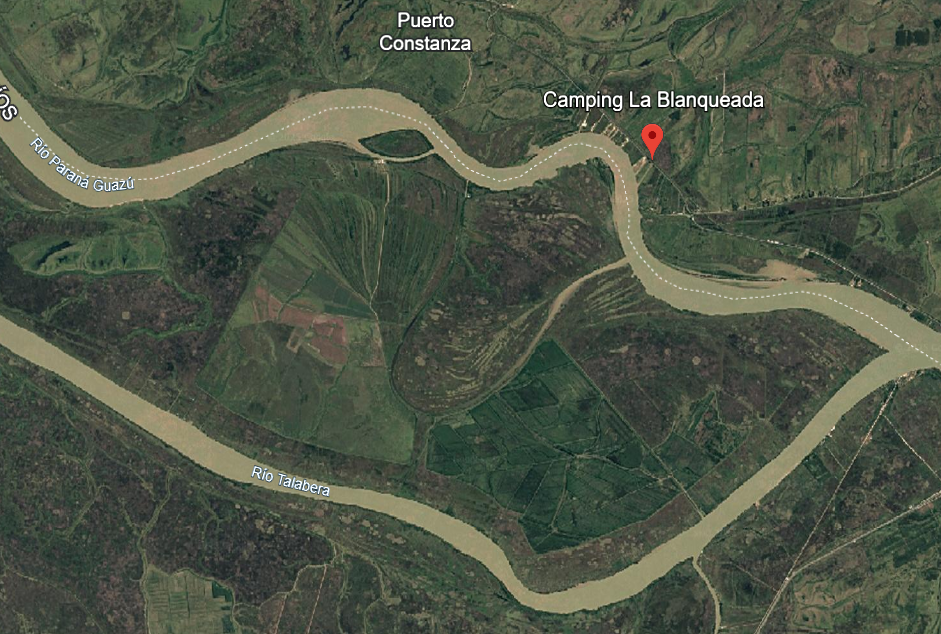
\includegraphics[width=0.70\linewidth]{figures/ch5/Camping Blanqueada.png}
    \caption{Location of camping La Blanqueada \autocite{googleGoogleEarth2025}}
    \label{fig:Camping Blanqueada}
\end{figure}

This would allow for a comparison with satellite data obtained in the future from software such as Aqua Monitor from Deltares. This software was used to alert critical erosion points along the Paraná Guazú in a broader scale. After the first map data was obtained from the satellite imagery, it was deemed necessary to investigate actual areas and lengths of land that have been subject to water gains and losses. Then the precise location of coast erosion was in turn analysed using Google Earth. The satellite database of Deltares was used for different time stamps, starting from 1984. The reason behind this is that the Deltares Aqua Monitor contains satellite imagery from 1984 until today. The choice was made to analyse the data in time batches of 10 years from 1985 until 2005, then in 5 years from 2005 to 2015, and lastly every 2.5 years in the last decade.

A preview of the maps can be seen in Figure \ref{Aqua Monitor Water Changes 1985-2025}, but the final analysis and conclusions are explained in Chapter \ref{chap:hydroanalysis}. The green parts indicate water losses and the blue parts show water gains over time. For the whole collection of figures, see Appendix \ref{Appendix: Satellite Data}.

\begin{figure}[H]
    \centering
    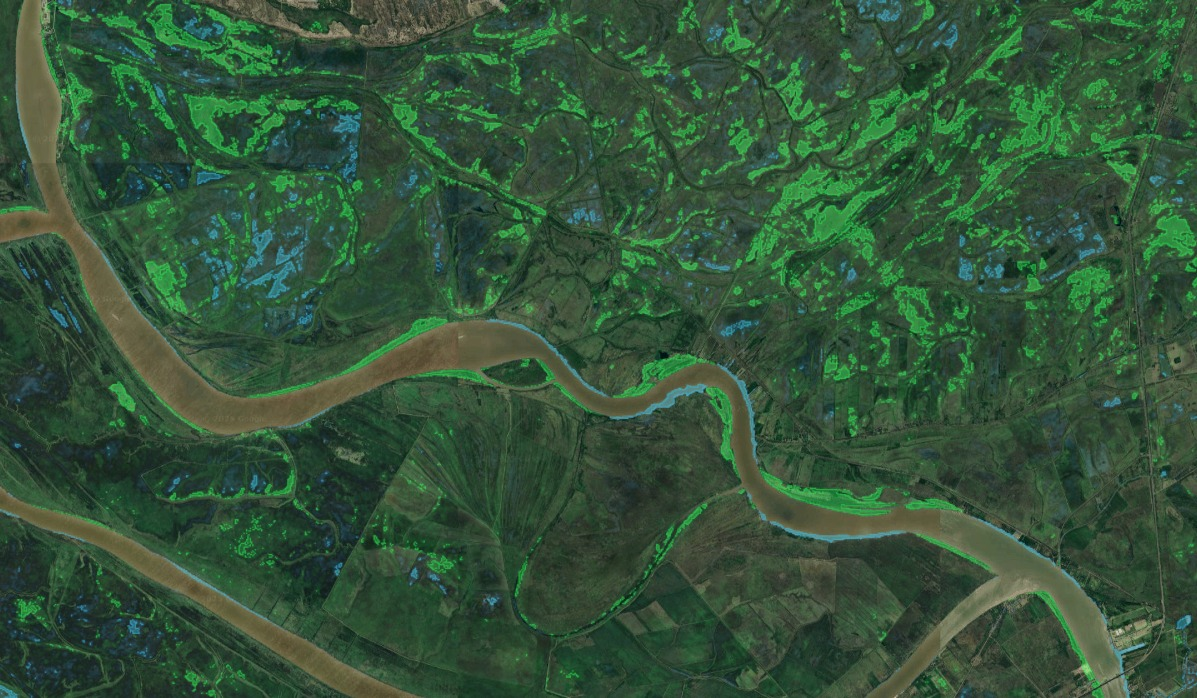
\includegraphics[width=0.75\linewidth]{figures/ch4/1985-2025.jpg}
    \caption{Aqua Monitor water surface changes over the period 1985-2025 \autocite{googleGoogleEarth2025}}
\end{figure}
\label{Aqua Monitor Water Changes 1985-2025}

\section{Modelling approach}
This section explains the approach for the models used in the report. Firstly, a two-dimensional hydrodynamic model was set up in Delft3D software. The model was designed to simulate flow velocities, water levels, and bed shear stresses in the confluence area where dredging activities take place. Delft3D was selected because it provides a robust framework to simulate complex river systems, while maintaining computational efficiency.

The model setup is described in Chapter \ref{chap:Delft3DModel}, including the generation of the bathymetry and computational grid. The hydrological inputs were based on field measurements taken during the campaign of 25–26 September 2025, complemented by discharge data from a one-dimensional HEC-RAS model provided by INA. Model calibration and sensitivity analyses were conducted to examine the influence of roughness and turbulence parameters on the simulated hydrodynamics and to evaluate model robustness. The resulting Delft3D simulations provided spatially detailed insight into the flow structure, highlighting high-velocity zones, areas of recirculation, and regions with elevated bed shear stresses.

Secondly, a sheet pile model was developed. This resulted in a design that acts as a mitigation strategy against bank erosion. Prior to designing this specific solution, an overview of structural mitigation measures was compiled, and all potential options were evaluated. Subsequently, the design for the selected solution (sheet pile) was created. A flow chart was used to outline the modelling methodology. The flow chart shown in Figure \ref{fig:flow_chart} is divided into three phases. In the first phase, data analysis, literature research was performed to gain a better understanding of the critical locations and parameters necessary for the design. First of all, geological soil conditions including borehole findings were used to assess the different layers and the accompanying soil parameters. Further, hydraulic parameters including bathymetry were provided by INA to assess water level and river bed formation along the banks and finally, structural standards and regulations, the Eurocode, were used to perform structural verifications regarding the ultimate limit and the serviceability limit state.

In the second phase of the model, a sheet pile type was chosen and the gathered data was used to analyse the earth and hydrostatic pressures. Multiple design methods were reviewed, and finally the simplified Padfield and Mair method was chosen to perform the earth and hydraulic pressure analysis. The procedure for calculating the embedding depth of the sheet pile came from the simplified Padfield and Mair method, and the pressure diagrams for the earth and hydrostatic pressure were analysed in Python. By combining the earth and hydrostatic pressures, the balance of moments and the final embedding depth were calculated. Then, the acting components such as shear, bending, and shear buckling were compared to the resistance of the chosen sheet pile profile to access the safety of the design. The final phase includes structural verification of the profile and design, along with drawing of the final sheet pile design.

\begin{landscape}
\thispagestyle{empty}
    \begin{figure}[H]
        \centering
        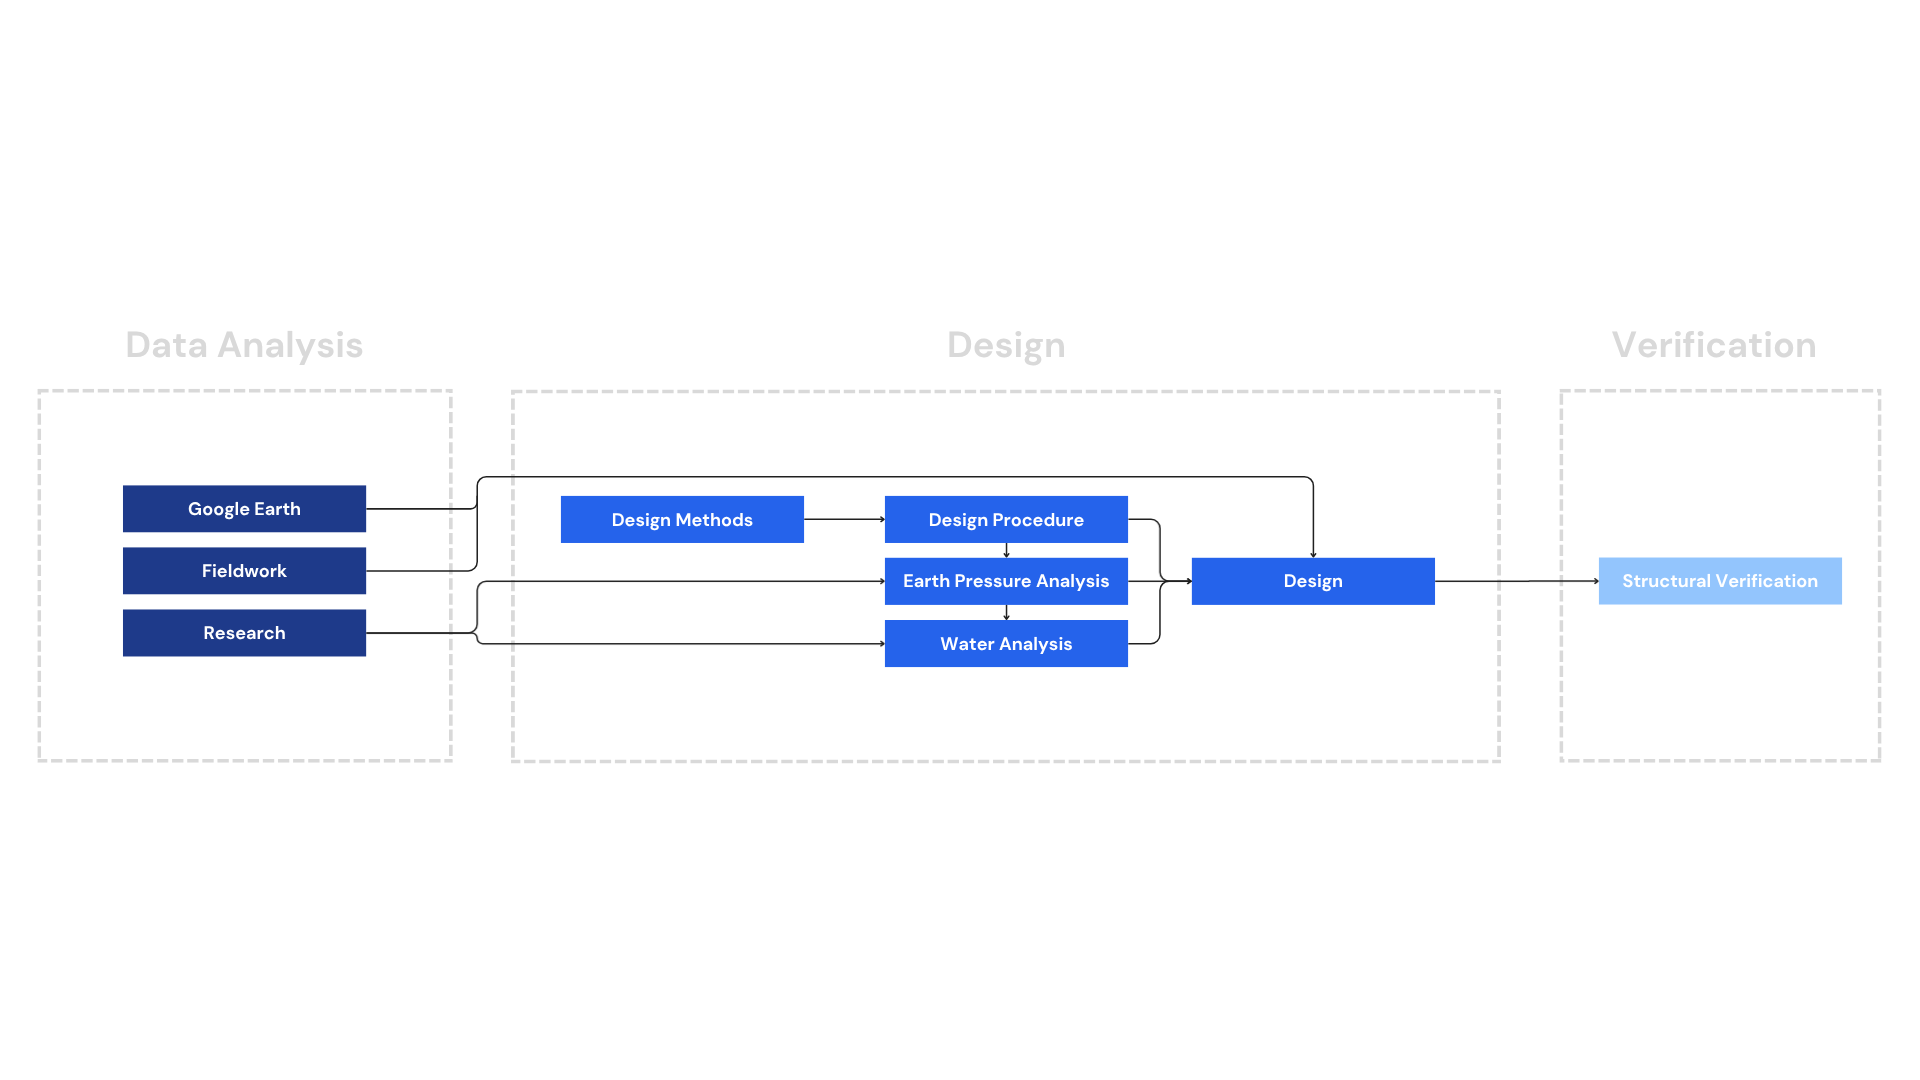
\includegraphics[width=1.2\linewidth]{figures/ch3/FlowChart Structural (4).png}
        \caption{Flow chart sheet pile model}
        \label{fig:flow_chart}
    \end{figure}
\end{landscape}